\documentclass{article}
% preamble 
  \usepackage[letterpaper, top=1in, bottom=1in, left=1in, right=1in]{geometry}
  \usepackage[utf8]{inputenc}
  \usepackage[english]{babel}
  \usepackage{amsmath, amssymb, amsthm, mathtools} % necessary 
  \usepackage{lastpage} % insert last page number 
  \usepackage{centernot} % for not slash 

  \usepackage{pgfplots}
  \pgfplotsset{compat=1.18}
  \usepackage{hyperref} % hyperlinks 
  \usepackage{fancyhdr} % fancy headers 
  \usepackage{fancyvrb} % verbatim 
  \usepackage{parskip}

  \usepackage{subcaption} % captions for figures 
  \definecolor{cverbbg}{gray}{0.93}

  \setlength{\parindent}{0pt} % set no indent
  \hfuzz=5.002pt % ignore overfull hbox badness warnings below this limit

  \DeclareMathOperator{\Tr}{Tr}
  \DeclareMathOperator{\Sym}{Sym}
  \DeclareMathOperator{\Span}{span}
  \DeclareMathOperator{\std}{std}
  \DeclareMathOperator{\Cov}{Cov}
  \DeclareMathOperator{\Var}{Var}
  \DeclareMathOperator{\Corr}{Corr}
  \DeclareMathOperator*{\argmin}{\arg\!\min}
  \DeclareMathOperator*{\argmax}{\arg\!\max}
  \newenvironment{question}{\color{blue}}{\ignorespacesafterend}


  \newcommand{\ket}[1]{\ensuremath{\left|#1\right\rangle}}
  \newcommand{\bra}[1]{\ensuremath{\left\langle#1\right|}}
  \newcommand{\bracket}[2]{\langle #1 | #2 \rangle}
    
  \theoremstyle{definition}
  \newtheorem{theorem}{Theorem}[section]
  \newtheorem{proposition}[theorem]{Proposition}
  \newtheorem{lemma}[theorem]{Lemma}
  \newtheorem{example}{Example}[section]
  \newtheorem{exercise}{Exercise}[section]
  \newtheorem{corollary}{Corollary}[theorem]
  \newtheorem{definition}{Definition}[section]
  \renewcommand{\qed}{\hfill$\blacksquare$}
  \renewcommand{\footrulewidth}{0.4pt}% default is 0pt
  
  \newenvironment{solution}{\noindent \textit{Solution.}}{}
  \newenvironment{cverbatim}
    {\SaveVerbatim{cverb}}
    {\endSaveVerbatim
    \flushleft\fboxrule=0pt\fboxsep=.5em
    \colorbox{cverbbg}{%
      \makebox[\dimexpr\linewidth-2\fboxsep][l]{\BUseVerbatim{cverb}}%
    }
    \endflushleft
  }

  \renewcommand{\thispagestyle}[1]{} % needed for including header in title page

\begin{document}
\pagestyle{fancy}

\lhead{Quantum Computing}
\chead{Muchang Bahng}
\rhead{\date{Spring 2024}}
\cfoot{\thepage / \pageref{LastPage}}

\title{Quantum Computing}
\author{Muchang Bahng}
\date{Spring 2024}

\maketitle
\tableofcontents
\pagebreak 

Notes from Neilson and Chuang.

\section{Fundamentals}

  In here we provide the foundations to work with quantum computing by introducing quantum mechanics and basic principles. A good amount of linear algebra should be known. I list some relevant concepts: 
  
  \begin{enumerate}
    \item Adjoint operators and Hilbert spaces 
    \item Tensor products
    \item Eigendecomposition 
    \item Commutators and Anit-commutators 
    \item SVD and Polar Decomposition 
  \end{enumerate}

  \subsection{Postulate 1: State Space}

    In quantum mechanics we usually work in a Hilbert space $V$ over field $\mathbb{C}$. A \textbf{ket} is of the form $| v \rangle$, which mathematically denotes a vector $v$ in $V$. A \textbf{bra} is of the form $\langle f |$, which denotes a covector $f \in V^\ast$, the dual space. With the usual construction of the canonical isomorphism between a Hilbert space and its dual, we say if $| m \rangle$ defines a column vector in $\mathbb{C}^n$, then $\langle m |$ is its conjugate transpose. This is formalized in the first postulate. 

    \begin{theorem}[Postulate 1: State Space]
      Associated to any isolated physical system is a Hilbert space (a complex inner product space) known as the \textbf{state space} of the system. The system is completely described by its \textbf{state vector}, which is a unit vector in the system's state space. 
      \begin{equation}
        \ket{\psi} \in \mathcal{H} \text{ s.t. } \bracket{\psi}{\psi} = 1 
        \label{eq:state_vector}
      \end{equation}
        
      This has been stated in a general term without respect to any basis. However, if we do fix an orthonormal basis $\mathcal{B} = \{\ket{\psi_1}, \ldots, \ket{\psi_n}\}$, then the state can be written in the form 
      \begin{equation}
        \ket{\psi} = \sum_{j=1}^D \alpha_j \ket{\psi_j}, \text{where} \sum_{j} |\alpha_j|^2 = 1 
        \label{eq:pos_1}
      \end{equation}

      The basis with which we write $\ket{\psi}$ with respect to is important when we perform measurement operators on it, as we will see later. 
    \end{theorem}

    This postulate is quite intuitive, since in Lagrangian mechanics we use the familiar configuration manifold to model the state of a system, and by Whitney's embedding theorem every manifold can be embedded in a sufficiently high-dimensional vector space. But QM does not tell us what the state space of that system is, nor does it tell us what the state vector of that system is. Figuring it out for a specific system is done independently with rules that physicists have developed. Furthermore, as we will see later, the choice of base relates to possible measurements of the system, and each base is associated with a particular measurement (or a group of compatible measurements). 
    \par 

    The most fundamental construct of computer science is the bit, which is $0$ or $1$. This is intuitive, since it is easy to understand mathematically and it also has an easy physical realization. For example, when computers retrieve memory or when you have a wire with some electrical current flowing over a certain threshold. The quantum analogue of the bit and the simplest quantum mechanical system is a single qubit. While the physical realization is less intuitive, let's only focus on the mathematical construct and properties for now. 

    \begin{definition}[Basis States]
      We list 4 different orthonormal bases that we will work with often in $\mathbb{C}^2$. We first introduce the standard basis, the Z basis state, and write the rest of the states in the Z basis. 

      \begin{enumerate}
        \item The classical notions of the $0$ and $1$ bit can be represented as the orthonormal vectors $\ket{0}, \ket{1} \in \mathbb{C}^2$, called \textbf{computational basis states} or the \textbf{z basis states}, which are
          \[\ket{0} = \ket{+}_z = \begin{pmatrix} 1 \\ 0 \end{pmatrix}, \;\;\;\; \ket{1} = \ket{-}_z = \begin{pmatrix} 0 \\ 1 \end{pmatrix}\]  

        \item The \textbf{x basis states} are 
          \begin{equation}
            \ket{+}_x \coloneqq \frac{\ket{0} + \ket{1}}{\sqrt{2}} , \;\;\;\; \ket{-}_x \coloneqq \frac{\ket{0} - \ket{1}}{\sqrt{2}} 
            \label{eq:x_basis}
          \end{equation}
        
        \item The \textbf{y basis states} are 
          \begin{equation}
            \ket{+}_y \coloneqq \frac{\ket{0} + i \ket{1}}{\sqrt{2}} , \;\;\;\; \ket{-}_y \coloneqq \frac{\ket{0} - i \ket{1}}{\sqrt{2}} 
            \label{eq:y_basis}
          \end{equation}
      \end{enumerate}      
    \end{definition}


    \begin{definition}[Qubit]
      A \textbf{qubit} is simply a vector $\ket{\psi} \in \mathbb{C}^2$. The natural orthonormal basis for this vector space is the computational basis states, but given any orthonormal basis $\mathcal{B} = \{\ket{\psi_1} , \ket{\psi_2}\}$, we can write the qubit as a linear combination of them, known as a \textbf{superposition}. Note that since $\ket{\psi}$ is unit, its coefficients with respect to every basis must satisfy the normalization.  

        \[\ket{\psi} = \alpha \ket{\psi_1} + \beta \ket{\psi_2} = \begin{pmatrix} \alpha \\ \beta \end{pmatrix}, \text{ where } |\alpha|^2 + |\beta|^2 = 1\]

      When we measure this qubit, for now we can interpret it has a $|\alpha|^2$ probability of realizing into the result $0$ and $|\beta|^2$ probability of realizing into $1$ (this notion is formalized in postulate 3). The coefficients of the state vector are also called the \textbf{amplitude}. 
    \end{definition} 

    \begin{example} 
      Say that a qubit with respect to the standard basis can be written as 
      \begin{equation}
        \ket{\psi} = \alpha \ket{0} + \beta \ket{1}
        \label{eq:qubit_standard_basis}
      \end{equation}
      Then, we can write it with respect to another basis as 
      \begin{equation}
        \ket{\psi} = \alpha \frac{\ket{+} + \ket{-}}{\sqrt{2}} + \beta \frac{\ket{+} - \ket{-}}{\sqrt{2}} = \frac{\alpha + \beta}{\sqrt{2}} \ket{+} + \frac{\alpha - \beta}{\sqrt{2}} \ket{-}
        \label{eq:qubit_not_standard_basis}
      \end{equation}
      which we can interpret as having a probability of $|\alpha + \beta|^2 /2$ of realizing to $\ket{+}$ and probability of $|\alpha - \beta|^2 / 2$ of realizing to $\ket{-}$. This may not make sense since we just said that it has a probability of $|\alpha|^2$ and $|\beta|^2$ of realizing to $\ket{0}$ and $\ket{1}$, but these probabilities emerge depending on the basis when we measure.  
    \end{example}

  \subsection{Postulate 2: Evolution}

  The equations of motion of a physical system can be written as a differential equation relating the derivative of the position vector $\ket{\psi(t)}$ with some operator on $\ket{\psi(t)}$. This operator can be a simple linear map $A$, leading to a \textbf{time-independent} equation of form
    \begin{equation}
      \frac{d}{dt} \ket{\psi(t)} = A \ket{\psi(t)} 
      \label{eq:form }
    \end{equation}
    Sometimes, it may be \textbf{time-dependent}, meaning that the operator $A$ can also change with time, and so we should replace it above with $A(t)$. For now, we will focus on the time-independent equation. 

    \begin{definition}[Schrodinger's Equation of Motion]
      The time evolution of a closed quantum system is described by the \textbf{Schrodinger equation}

        \[i \hbar \frac{d |\psi \rangle}{dt} = \hat{H} |\psi \rangle, \]

      an ordinary differential equation with solution $| \psi \rangle (t)$ ($|\psi\rangle: \mathbb{R}_t \longrightarrow \mathbb{C}^n$, the Hilbert space). Where $\hbar$ is Planck's constant and $\hat{H}$ is a fixed Hermitian operator called the \textbf{Hamiltonian} of the closed system. Note that because $H$ is self-adjoint, it has the spectral decomposition

        \[H = \sum_{E} E \, |E \rangle \langle E |\]

      with eigenvalues $E$ and corresponding normalized eigenvectors $|E \rangle$. The eigenvectors $|E \rangle$ are called \textbf{energy eigenstates} with the energy of the state being $E$. The minimum energy and energy eigenstate is known as the \textbf{ground state energy} and \textbf{ground state}, respectively.
    \end{definition}

    \begin{question} 
      Motivations of using a self-adjoint operator as the Hamiltonian? What do the energy levels (eigenvalues) and eigenvectors mean? How do we solve this equation of motion? 
    \end{question}

    The solutions to the time-indpendent Schrodinger's equation (with initial time value $t_1$ and its initial state vector $|\psi (t_1)\rangle$), which is easily verified to be:

    \begin{align*}
      |\psi (t_2) \rangle & = \exp \bigg( \frac{-i \hat{H} (t_2 - t_1)}{\hbar} \bigg) \, |\psi(t_1)\rangle \\
      & = U(t_1, t_2) \, |\psi (t_1) \rangle
    \end{align*}

    Since $U$ is the exponential of an imaginary scalar times the Hermitian operator, we can prove that it is unitary. The converse is also true: for every unitary operator there exists a Hermitian operator satisfying the identity above, and thus we can rewrite the dynamics of the time-independent Schrodinger's equation above to postulate 2. 
    
    \begin{theorem}[Postulate 2: Evolution]
      The evolution of a closed quantum system is described by a unitary transformation U. That is, the state of the system $|\psi \rangle$ at time $t_1$ is related to the state $|\psi^\prime \rangle$ of the system at time $t_2$ by a unitary operator $U$ which depends only on the times $t_1$ and $t_2$.

        \[|\psi^\prime \rangle = U \, |\psi \rangle\]
    \end{theorem}

    In general finding out the Hamiltonian of a system is a very difficult problem, but we will assume that it is given in our context. Furthermore, for systems that are under the experimentalist's control and which may be changed, a \textbf{time-varying Hamiltonian} may be used to describe the quantum system. 

    We have postulated that closed quantum systems evolve according to unitary evolution. The evolution of systems which don't interact with the rest of the world is all very well, but there must also be times when the experimenter and their experimental equipment (i.e., an external physical system) observe the system to find out what is going on inside the system. This observation is an interaction with the system, making the system not closed, and thus not subject to unitary evolution. The effects of measurements done on quantum systems can be described with postulate 3, and in here let us remind the reader that a measurement outcome is \textit{different} than the state of a quantum system (e.g., the state space of a qubit is the complex $2$-sphere, while the measurement outcomes can be $0$ or $1$).

    \subsubsection{Logic Gates}

      From postulate 2, we have found out that closed quantum systems evolve according to a unitary operator. A question to ask is what kind of unitary operators are natural to consider? In the case of single qubits, it turns out that \textit{any} unitary operator at all can be realized in physical systems. Therefore, we can modify these qubits with general unitary operators, which are in some way a generalization of classical logic gates. Quantum logic gates can be interpreted as matrices that modify the state of qubits. This is similar to those of classical gates, but one key difference between quantum logic gates and classical ones is that quantum gates are always invertible (from the unitary condition), while some classical gates like NAND are irreversible (e.g., if the output of a NAND gate is $1$, we don't know if the input is $00, 01$, or $10$). We can divide them into classes depending on how many arguments they take, but as we will see, the general form of a quantum gate taking in $n$ input qubits is some unitary matrix in $U(2^n)$. Let us first focus on gates of one qubit. We will start with the Pauli matrices and spend some time investigating their properties.  

      \begin{definition} 
        The \textbf{Pauli matrices} are defined 
          \[
            X = \begin{pmatrix} 0 & 1 \\ 1 & 0 \end{pmatrix},  
            Y = \begin{pmatrix} 0 & -i \\ i & 0 \end{pmatrix},   
            Z = \begin{pmatrix} 1 & 0 \\ 0 & -1 \end{pmatrix}  
          \]
      \end{definition}

      \begin{question}
        Can we use Pauli matrices on other orthonormal bases?  
      \end{question}

      \begin{lemma}[Decomposition of Pauli Matrices]
        The Pauli matrices are self-adjoint (Hermitian) and unitary. 
      
        \begin{enumerate}
          \item They have the outer product decomposition of: 

            \[X = \ket{1} \bra{0} + \ket{0} \bra{1}, Y = i \ket{1} \bra{0} - i \ket{0} \bra{1}, Z = \ket{0} \bra{0} - \ket{1} \bra{1}\]

          \item They have an eigendecomposition of: 

            \[\]

        \end{enumerate}

      \end{lemma}
      \begin{proof}
        To see that they're self adjoint, if you take the conjugate transpose they are the same. To see unitary, we can see that the columns are orthonormal. 
      \end{proof}

      \begin{theorem}
        These three matrices are very important because it turns out that

          \[\frac{1}{2} i X, \frac{1}{2} i Y, \frac{1}{2} i Z\]

        forms the basis for the Lie algebra $\mathfrak{u}(2)$, which exponentiates to the unitary group $\text{U}(2)$. Therefore, by exponentiating each Pauli matrix, we have

        \begin{align*}
          e^{-i \beta X /2} &= \cos \frac{\beta}{2} I - i \sin \frac{\beta}{2} X = \begin{pmatrix} \cos \frac{\beta}{2} & -i \sin \frac{\beta}{2} \\ -i \sin \frac{\beta}{2} & \cos \frac{\beta}{2} \end{pmatrix}, \\
          e^{-i \gamma Y/2} &= \cos \frac{\gamma}{2} I - i \sin \frac{\gamma}{2} Y = \begin{pmatrix} \cos \frac{\gamma}{2} & - \sin \frac{\gamma}{2} \\ \sin \frac{\gamma}{2} & \cos \frac{\gamma}{2} \end{pmatrix}, \\
          e^{-i \delta Z/2} &= \cos \frac{\delta}{2} I - i \sin \frac{\delta}{2} Z = \begin{pmatrix} e^{-i \delta /2} & 0 \\ 0 & e^{i\delta/2} \end{pmatrix}.
        \end{align*}

        and so every rotation matrix $U \in \text{U}(2)$, which represents single qubit operations, can be decomposed as the following products for real values of $\beta, \gamma, \delta$:

        \[
          U = \begin{pmatrix} \cos \frac{\beta}{2} & -i \sin \frac{\beta}{2} \\ -i \sin \frac{\beta}{2} & \cos \frac{\beta}{2} \end{pmatrix} \begin{pmatrix} \cos \frac{\gamma}{2} & - \sin \frac{\gamma}{2} \\ \sin \frac{\gamma}{2} & \cos \frac{\gamma}{2} \end{pmatrix} \begin{pmatrix} e^{-i \delta /2} & 0 \\ 0 & e^{i\delta/2} \end{pmatrix}.
        \]
      \end{theorem}

      \begin{theorem}[Commutation and Anti-Commutation]
        The Pauli matrices satisfy the following properties. 
        \begin{enumerate}
          \item Commutation properties: 
           

          \item Anticommutation properties: 


        \end{enumerate}
      \end{theorem}

      Now we introduce other operators. 

      \begin{definition}
        Listed. 

        \begin{enumerate}
          \item The \textbf{Hadamard gate} $H$ takes in $|0\rangle$ or $|1\rangle$ and puts it into exactly equal superposition.

            \[H = \frac{1}{\sqrt{2}} \begin{pmatrix} 1 & 1 \\ 1 & -1 \end{pmatrix}.\]

          That is, $H|0\rangle = |+\rangle$ and $H|1\rangle = |-\rangle$. This can be thought of as a rotation around the Bloch vector $(1, 0, 1)$.

          \item The \textbf{Phase gate} $S$ is the square root of the Pauli-Z gate.

            \[S = \begin{pmatrix} 1 & 0 \\ 0 & i \end{pmatrix}.\]

          \item The \textbf{$\pi/8$ gate} $T$ is the square root of the Phase gate.

            \[T = \begin{pmatrix} 1 & 0 \\ 0 & e^{i \pi/4} \end{pmatrix}.\]
        \end{enumerate} 
      \end{definition}

      
  \subsection{Postulate 3: Measurement}

    We have postulated that closed quantum systems evolve according to unitary evolution, but there must be times when the experimentalist must interact with the external system through some measurement. To explain what happens when this is one, we use postulate 3, which provides a means for describing the effects of measurements on quantum systems. 

    \begin{theorem}[Posulate 3: General Measurement]
      Given a state vector $\ket{\psi} \in \mathcal{H}$ with a total possible number of measurement outcomes parameterized by $m$. Then, a quantum measurement is described by a collection $\{M_m\}$ of \textbf{measurement operators} (acting on the state space) satisfying the \textit{completeness equation}

        \[\sum_{m} M_m^\dagger M_m = I\]

      If the state of the quantum system is $|\psi \rangle$ immediately before the measurement, then the probability that result $m$ occurs is

        \[p(m) = \langle \psi | M_m^\dagger M_m | \psi \rangle\]

      Immediately after this measurement outcome $m$, the state of the system then becomes

        \[\frac{M_m |\psi \rangle}{\sqrt{\langle \psi| M_m^\dagger M_m |\psi \rangle}} = \frac{M_m |\psi \rangle}{\sqrt{p(m)}}\]

      Note that the completeness equation implies

        \[1 = \sum_m p(m) = \sum_m \langle \psi | M_m^\dagger M_m | \psi \rangle\]

      Note that we have defined measurements in a basis-independent way. If we do fix an orthonormal $B = \{ \ket{\psi_1}, \ldots, \ket{\psi_n}\}$, then both the state $\ket{\psi}$ and the measurement operators $\{M_m\}$ should be written with respect to $B$. 

    \end{theorem}

    \begin{question} 
      What is the physical realization of a measurement operator? 

      We've defined in a basis independent way, but when conducting measurements, we must choose an orthonormal basis $v_1, v_2$. Now does the measurement operator have to be in that same basis? (probably yes). Next question is what does the eigenvectors (which should be orthonormal) have to do with it? Are the possible outcomes determined to be the fixed bases or the eigenvectors? 
    \end{question}

    That's all there is to measurements: they are a collection of operators satisfying the normalization identity above. Usually, this is not how measurement operators are introduced in quantum mechanics courses. They are introduced as projective measurements which can be encoded in self-adjoint operators, but for more precise measurements needed in quantum computing, we should introduce the generalized version first. 

    
    \begin{example}
      As an example, suppose that we have the simple quantum system consisting of a single qubit that has the state $|\psi \rangle = a|0\rangle + b|1 \rangle$  (w.r.t. Z basis) immediately before measurement

        \[\{M_0, M_1\} = \bigg\{ \begin{pmatrix} 0.8 & 0 \\  0 & 0.6 \end{pmatrix}, \; \begin{pmatrix} 0.6&0\\0&0.8 \end{pmatrix} \bigg\}\]

      which clearly satisfies the completeness equation $M_0^\dagger M_0 + M_1^\dagger M_1 = I$, has probabilities

      \begin{enumerate}
        \item $p(0) = \langle \psi | M_0^\dagger M_0 | \psi \rangle = 0.64 a^2 + 0.36b^2$ chance of a measurement outcome of $0$
        \item $p(1) = \langle \psi | M_1^\dagger M_1 | \psi \rangle = 0.36 a^2 + 0.64b^2$ chance of a measurement outcome of $1$
      \end{enumerate}

      If we observe a measurement of $0$ in the system, then the state vector of the quantum system would be

        \[\frac{M_0 | \psi\rangle}{\sqrt{\langle \psi | M_0^\dagger M_0 | \psi\rangle}} = \frac{1}{\sqrt{0.64a^2 + 0.36b^2}} \begin{pmatrix} 0.8a \\ 0.6b \end{pmatrix} = \frac{0.8a}{\sqrt{0.64a^2 + 0.36b^2}}\, |0 \rangle + \frac{0.6 b}{\sqrt{0.64a^2 + 0.36b^2}} \, |1\rangle\]

      and if we observe an outcome of $1$, then the state vector of the system would be

        \[\frac{M_1 | \psi\rangle}{\sqrt{\langle \psi | M_1^\dagger M_1 | \psi\rangle}} = \frac{1}{\sqrt{0.36a^2 + 0.64b^2}} \begin{pmatrix} 0.6a \\ 0.8b \end{pmatrix} = \frac{0.6a}{\sqrt{0.36a^2 + 0.64b^2}}\, |0 \rangle + \frac{0.8 b}{\sqrt{0.36a^2 + 0.64b^2}} \, |1\rangle\]
    \end{example}

    \begin{theorem}[Composition of Measurements]
    A following theorem is that a composition of measurements, e.g., $\{L_l\}$ followed by a separate $\{M_m\}$ is physically equivalent to a single measurement defined by measurement operators $\{N_{lm}\}$ with the representation $N_{lm} = M_m L_l$.  
    \end{theorem}

    \subsubsection{Bloch Sphere: Global and Relative Phase}

      Now that we've talked about measurements, we can introduce the global and relative phase, which will give us the justification to introduce the Bloch sphere. 


      \begin{definition}[Global and Relative Phase]
        Note that the unit sphere in $S^2 \subset \mathbb{C}^2$ captures the state space of the single qubit in full generality. Because $|\alpha|^2 + |\beta|^2 = 1$, we can rewrite the qubit to 

        \begin{equation}
          \ket{\psi} = \alpha \ket{0} + \beta \ket{1} = e^{i \gamma} \bigg( \cos{\frac{\theta}{2}} \ket{0} + e^{i \varphi} \sin{\frac{\theta}{2}} \ket{1} \bigg) 
          \label{eq:global_phase}
        \end{equation}

        where $\theta, \gamma, \varphi \in \mathbb{R}$. The $e^{i \gamma}$ is known as the \textbf{global phase} and $e^{i \varphi}$ is known as the \textbf{relative phase}. 
      \end{definition}

      Now note that $\ket{\psi}$ and $e^{- i \gamma} \ket{\psi}$ are two different states in $S^2$. Let us measure them with a set of measurements $\{M_m\}$, and we can see that they both give the same probabilities for each outcome $m$. 
      
      \begin{align*}
        p(m) & = \langle e^{i \delta} \psi | M_m^\dagger M_m | e^{i \delta} \psi \rangle, \\
        & = \langle \psi | e^{-i \delta} M_m^\dagger M_m e^{i \delta} | \psi \rangle, \\
        & = \langle \psi | M_m^\dagger M_m | \psi \rangle = p(m)
      \end{align*}

      Therefore, both $\ket{\psi}$ and any state vector of form $e^{i \gamma} \ket{\psi}$ produce the same probabilities under any general measurement, and from an observational point of view, these two states are identical. So we can construct a quotient space on $S^2$ by defining a equivalence relation $\ket{\psi} \sim e^{i\gamma} \ket{\psi}$ where both are equal up to a global phase factor. This restricts our states space to having 2 real parameters $\theta$ and $\varphi$, so we now can construct some visual. 

      \begin{definition}[Bloch Sphere]
        The previous parameterization of the real unit sphere $S^2 \subset \mathbb{R}^2$ is known as the \textbf{Bloch sphere}, which can be visualized below. 

        \begin{center}
          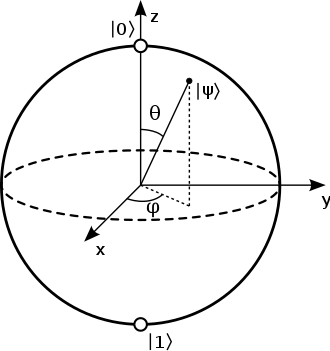
\includegraphics[scale=0.4]{img/330px-Bloch_sphere.png}
        \end{center}


        A few properties should be mentioned: 
        \begin{enumerate}
          \item The antiparallel vectors lying on the $X, Y, Z$ axes represent the orthonormal $X, Y, Z$ basis in $\mathbb{C}^2$. Note that while the basis is pairwise perpendicular in $\mathbb{C}^2$, in the Bloch sphere they are visualized as antiparallel. 

          \item The probability of it being $|0\rangle$ or $|1\rangle$ depends on the value of $\theta$. 
        \end{enumerate}
      \end{definition}

      



      The other kind of phase is known as the \textbf{relative phase factor}. Given two states

        \[|\psi \rangle = \alpha |0\rangle + \beta |1\rangle \text{ and } |\psi^* \rangle = \alpha^* |0 \rangle + | \beta^* \rangle,\]

      if $|\alpha| = |\alpha^*|$ or $|\beta| = |\beta^*|$, then we say that \textbf{the amplitudes differ by a relative phase}. Furthermore, two states $|\psi \rangle, |\psi^* \rangle$ are said to \textbf{differ by a relative phase in some basis} if each of the amplitudes in that basis is related by such a phase factor. For example, two states 

      \[\frac{|0\rangle + |1\rangle}{\sqrt{2}} \text{ and } \frac{|0\rangle - |1\rangle}{\sqrt{2}}\]
      differ by a relative phase (in the computational basis $|0\rangle, |1\rangle$) since the $|0\rangle$ amplitudes differ by a relative phase factor of $1$ ($ \frac{1}{\sqrt{2}} = 1 \cdot \frac{1}{\sqrt{2}}$) and the $|1\rangle$ amplitudes differ by a relative phase factor of $-1$ ($-\frac{1}{\sqrt{2}} = -1 \cdot \frac{1}{\sqrt{2}}$). It is clear that due to Born's rule on this one-qubit system, $|\alpha| = |\alpha^*| \iff |\beta| = |\beta^*|$, and so, all we have to do is check the magnitudes of the $|0\rangle$ amplitudes of two state vectors. Visualizing this on the Bloch sphere, we can see that the $\theta$ is the only parameter capable of changing the $|0\rangle$ amplitude. The global phase factor $e^{i\gamma}$ is merely a rotation map and also cannot change the $|0\rangle$. Therefore, we can see that two state vectors differ by a relative phase if and only if they have the same $\theta$ value, i.e. if the two points on the Bloch sphere are on the same "latitude."

      \begin{center} 
        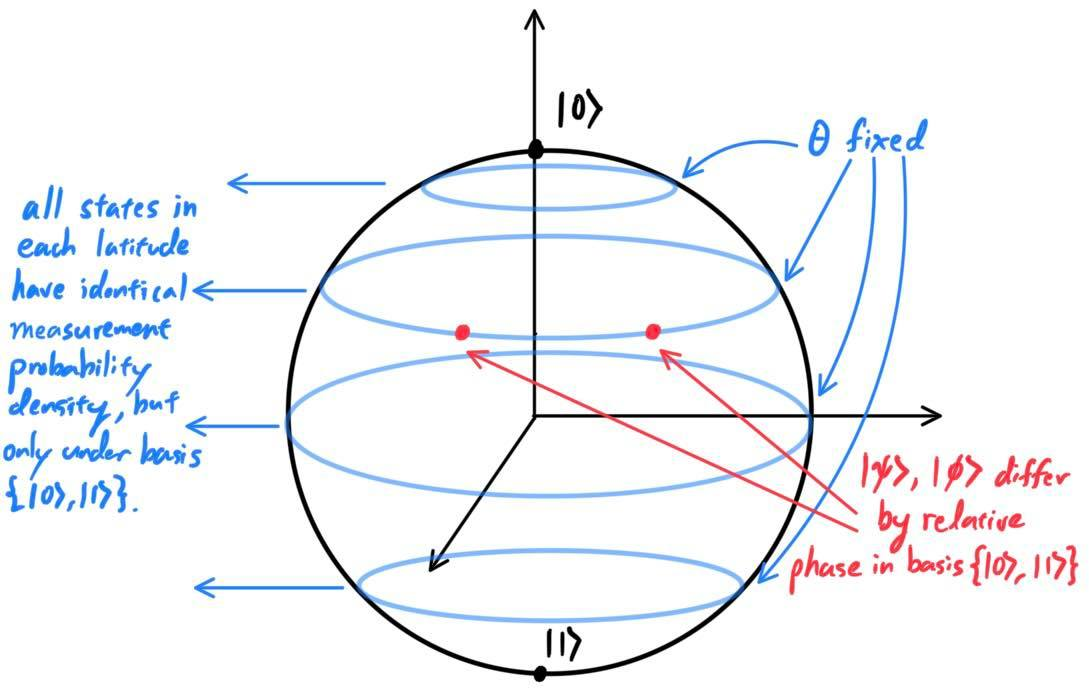
\includegraphics[scale=0.3]{img/Bloch_Sphere_latitude.jpg}
      \end{center}

      Notice that if two states are differ by a relative phase, then these phases are observationally equivalent, and so must be similar to the global phase factor. However, the relative phase is basis-dependent and so may produce different probability densities depending on the computational basis, while the global one is basis-independent. 

    \subsubsection{Projective Measurements}

      We have defined a measurement as a collection $\{ M_m\}$ of operators satisfying the completeness equation. The majority of cases that we will be interested in are projective measurements, which are a specific case of general measurements. 

      \begin{definition}[Projective Measurement]
        The following statements are all equivalent:

        \begin{enumerate}
          \item A projective quantum measurement is described by a collection $\{P_m\}$ of measurement operators that are orthogonal/Hermitian projectors satisfying the completeness equation (which can be simplified using the linear algebra properties above):
            \[\sum_m P_m^\dagger P_m = \sum_m P_m^2 = \sum_m P_m = I\]
          \item A projective quantum measurement is described by an \textbf{observable} $M$, a Hermitian operator on the state space with the spectral decomposition
            \[M = \sum_m m P_m\]
          such that the $P_m$'s satisfy the completeness equation.
          \item A quantum measurement "in an orthonormal basis $|m\rangle$" means to conduct a projective measurement with projectors $P_m = |m \rangle \langle m |$. This is equivalent to the two above because given two orthonormal vectors $|m\rangle, |m^\prime \rangle$, we have
            \[P_{m^\prime} P_m = |m^\prime \rangle \langle m^\prime | m \rangle \langle m | = \begin{cases} 0 & m^\prime \neq m \\ |m \rangle \langle m | = P_m & m^\prime = m \end{cases}\]
          which implies that $P_m$ is projective. Since $P_m$ is the outer product of two identical vectors it is clearly Hermitian, and therefore $P_m$ is an orthogonal projection. Furthermore, by the linear algebra result above we can see that the $P_m = |m\rangle \langle m|$ satisfies the completeness equation.
        \end{enumerate}
      \end{definition}

      This formulation simplifies calculations. Upon measuring the state $|\psi\rangle$, the probability of getting result $m$ is

        \[p(m) = \langle \psi | P_m^\dagger P_m | \psi \rangle = \langle \psi | P_m | \psi \rangle \text{ with state after measurement } \frac{P_m  \ket{\psi}}{\sqrt{p(m)}}\]

      When we conduct a measurement of some quantum system, we can interpret $M$ in two very similar and connected ways:

      \begin{enumerate}
        \item $M$, the observable, is a Hermitian operator that decomposes into the projectors $P_m$ that determines the probabilities $p(m)$ of result $m$ occurring.
        \item $M$ is a random variable that generates an $m$ representative of an element in the outcome space, following some multinomial probability density $p(m)$ when we measure the system.
      \end{enumerate}

      Interpreting $M$ as this random variable, the expected measurement outcome is:

      \begin{align*}
        \mathbb{E}(M) & = \sum_m m\, p(m) \\
        & = \sum_m m \langle \psi | P_m | \psi \rangle \\
        & = \langle \psi | \bigg( \sum_m m P_m \bigg) \, | \psi \rangle \\
        & = \langle \psi | M | \psi \rangle \equiv \langle M \rangle
      \end{align*}

      with variance

      \begin{align*}
        \big( \Delta (M)\big)^2 & = \langle (M - \langle M \rangle )^2 \rangle \\
        & = \langle M^2 \rangle - \langle M \rangle^2
      \end{align*}

      \begin{example}
        Let us have a 1-qubit quantum system that is in the state

          \[|\psi \rangle = \frac{|0\rangle + |1 \rangle}{\sqrt{2}} = \begin{pmatrix} 1/\sqrt{2} \\ 1/\sqrt{2} \end{pmatrix}\]

        and we (projectively) observe it with the Pauli-Z operator. We can calculate it to have eigenvalue $+1$ with eigenvector $|0\rangle$ and eigenvalue $-1$ with eigenvector $|1\rangle$. The decomposition of $Z$ into its projective maps is

        \begin{align*}
          Z & = (+1) \, P_{+1} + (-1)\, P_{-1} \\
          & = (+1) \, \begin{pmatrix} 1&0\\0&0 \end{pmatrix} + (-1)\, \begin{pmatrix} 0&0\\0&1 \end{pmatrix}
        \end{align*}

        and so the probability of getting a measurement of $+1$ or $-1$ is

        \begin{align*}
          p(+1) & = \langle \psi | P_{+1} | \psi \rangle = \begin{pmatrix} \frac{1}{\sqrt{2}} & \frac{1}{\sqrt{2}} \end{pmatrix} \begin{pmatrix} 1&0\\0&0 \end{pmatrix} \begin{pmatrix} \frac{1}{\sqrt{2}} \\ \frac{1}{\sqrt{2}} \end{pmatrix} = \frac{1}{2} \\
          p(-1) & = \langle \psi | P_{-1} | \psi \rangle = \begin{pmatrix} \frac{1}{\sqrt{2}} & \frac{1}{\sqrt{2}} \end{pmatrix} \begin{pmatrix} 0&0\\0&1 \end{pmatrix} \begin{pmatrix} \frac{1}{\sqrt{2}} \\ \frac{1}{\sqrt{2}} \end{pmatrix} = \frac{1}{2}
        \end{align*}
      \end{example}

      \begin{example}
        The state space of a classical bit is $\{0, 1\}$. On the other hand, the state of a \textbf{quantum bit}, or a \textbf{qubit}, is the 3-dimensional unit sphere in $\mathbb{C}^2$. More specifically, the state of the qubit can be parameterized by two \textbf{complex amplitudes} $\alpha, \beta$ defining a complex unit linear combination, or \textbf{superposition}, of the 0 and 1 vectors

        \[|\psi \rangle = \alpha \,|0 \rangle + \beta \, | 1\rangle, \;\;\;\;\;\; \alpha, \beta \in \mathbb{C}, \; |\alpha|^2 + |\beta|^2 = 1.\]

        That is, the state of a qubit is a vector in a two-dimensional complex vector space, with the special states $|0\rangle$ and $|1\rangle$ known as \textbf{computational basis states} and form an orthonormal basis for this vector space. Quantum mechanics tells us that upon observing this qubit, its state will "collapse" onto a state of $0$ or $1$, with probabilities determined by \textbf{Born's rule}: Given qubit $|\psi \rangle = \alpha \,|0 \rangle + \beta \, | 1\rangle$,

        \begin{align*}
          \mathbb{P}(\text{collapse to } 0) & = |\alpha|^2, \\
          \mathbb{P}(\text{collapse to } 1) & = |\beta|^2.
        \end{align*}

        Note that this isn't a special "rule" at all. If we make a projective measurement of $M = I$, having decomposition

          \[M_1 = \begin{pmatrix} 1 & 0 \\ 0 & 0 \end{pmatrix}, \;\;\; M_2 = \begin{pmatrix} 0 & 0 \\ 0 & 1 \end{pmatrix},\]

        on this single qubit system with state vector $|\psi \rangle = \alpha |0\rangle + \beta |1 \rangle$, we get

        \begin{align*}
          p(0) & = \langle \psi | M_0^\dagger M_0 | \psi \rangle = \begin{pmatrix} \overline{\alpha} & \overline{\beta} \end{pmatrix} \begin{pmatrix} 1 & 0 \\ 0&0 \end{pmatrix} \begin{pmatrix} \alpha \\ \beta \end{pmatrix} = \overline{\alpha} \alpha = |\alpha|^2, \\
          p(1) & = \langle \psi | M_1^\dagger M_1 | \psi \rangle = \begin{pmatrix} \overline{\alpha} & \overline{\beta} \end{pmatrix} \begin{pmatrix} 0 & 0 \\ 0&1 \end{pmatrix} \begin{pmatrix} \alpha \\ \beta \end{pmatrix} = \overline{\beta} \beta = |\beta|^2.
        \end{align*}

        Note again that this strange property of the qubit "being" in a continuum of states until it is observed runs counter to our intuition. Despite this, qubits are decidedly real, and different physical systems can be used to realize qubits.
      \end{example}

    \subsubsection{Distinguishing Quantum States}

      One interesting property of measurements arises when \textbf{distinguishing quantum states}. In short, it turns out that if we are trying to find out whether a quantum system is in state A or state B, it is possible to find out by measuring it if and only if A and B are orthogonal (i.e., orthonormal since state vectors are unit vectors). Elaborating on this, let us have a quantum system with some mystery state vector that is chosen from a set of states $\{|\psi_i \rangle \}_{i=1}^n$. For the sake of explanation, we will say that this mystery state vector is $|\psi_k \rangle$, with $1 \leq i = k \leq n$ (but remember that this is not actually known). Is it possible to measure the system so that we can correctly identify the correct state $|\psi_k \rangle$ from the $|\psi_i\rangle$'s, i.e., find the value $i=k$?

      \begin{enumerate}
        \item If all the $|\psi_i \rangle$'s are orthonormal, then this is possible. We define measurement operators $M_i \equiv |\psi_i \rangle \langle \psi_i |$ for $i = 1, \ldots, n$, a final operator

          \[M_0 = \sqrt{I - \sum_{i\neq 0} |\psi_i \rangle \langle \psi_i |}\]

        These operators $\{M_i\}$ satisfy the completeness equation, and since

          \[p(i) \equiv \langle \psi_k | M_i | \psi_k \rangle = \langle \psi_k | \psi_i \rangle \langle \psi_i | \psi_k \rangle = \begin{cases} 1 & i = k \\ 0 & i \neq k \end{cases}\]

        all we have to do is observe the system according to set $\{M_i\}$, which will give the outcome $i=k$ with probability $1$.

        \item If the $|\psi_i\rangle$'s aren't orthonormal, then there is some nonzero probability that the system may be in another state, and we cannot determine for sure the index $k$ of $|\psi_k \rangle$.
      \end{enumerate}

    \subsubsection{POVM Measurements}

      The measurement postulate involves two elements: the probabilities of the measurement outcomes and the post-measurement state of the system. When we are concerned with only the probabilities (e.g., in the case of an experiment where the system is measured only once), it is useful to employ the POVM formalism. Suppose a measurement described by measurement operators $M_m$ is performed upon a quantum system in the state $|\psi\rangle$. Then, the probability of outcome $m$ is given by $p(m) = \langle \psi | M_m^\dagger M_m | \psi \rangle$. 

      We now define

        \[E_m \coloneqq M_m^\dagger M_m\]

      to be the \textbf{POVM elements} associated with the measurement, and the complete set $\{E_m\}$ to be the \textbf{POVM}. Some linear algebra reveals that $E_m$ must be positive-definite, the POVM is sufficient to completely determine the probabilities of the different measurement outcomes. For a projective measurement described by measurement operators $P_m$, we can see that they are equal to the POVM elements since $E_m \equiv P_m^\dagger P_m = P_m$.

      We have seen that the existence of a set of measurement operators $\{M_m\}$ satisfying the completeness equation automatically implies the existence of the POVM $\{E_M\}$ consisting of positive operators satisfying $\sum_m E_m = I$:

        \[\{M_m\} \longrightarrow \{E_m\}.\]

      Going backwards, we claim that the existence of an arbitrary set of positive operators $\{E_M\}$ satisfying $\sum_m E_m = I$ implies the existence of measurement operators $\{M_m\}$ defining a measurement described by the POVM. We simply define $M_m \equiv \sqrt{E_m}$, which we can do since $E_m$ is positive (define a new linear map with the same eigenspaces but square root of eigenvalues).

        \[\{M_m\} \longleftrightarrow \{E_m\}.\]

      The applicability of POVMs is demonstrated in the following example: Suppose a qubit is in one of two states: $|\psi_1 \rangle = |0 \rangle$ or $|\psi_2 \rangle = (|0 \rangle + |1 \rangle)/2$. Since these qubits are not orthonormal, we cannot determine the state with 100\% accuracy. However, it is possible for us to perform a measurement that distinguishes the states sometimes, but never makes an error of identification. We can construct a POVM of three elements as such:

      \begin{align*}
        E_1 & \equiv \frac{\sqrt{2}}{1 + \sqrt{2}} |1\rangle \langle 1| = \frac{\sqrt{2}}{1 + \sqrt{2}} \begin{pmatrix} 0&0\\0&1 \end{pmatrix}, \\
        E_2 & \equiv \frac{\sqrt{2}}{2 + 2 \sqrt{2}} \begin{pmatrix} 1 & -1 \\ -1 & 1 \end{pmatrix}, \\
        E_3 & \equiv I - E_1 - E_2.
      \end{align*}

      It can be checked that these sum up to $I$ and are positive definite. If the actual state of the system was $|\psi_1 \rangle$, then we have

      \begin{align*}
        p(1 \,|\, |\psi_1 \rangle) & = \langle \psi_1 | E_1 | \psi_1 \rangle = 0, \\
        p(2 \,|\, |\psi_1 \rangle) & = \langle \psi_1 | E_2 | \psi_1 \rangle = \frac{\sqrt{2}}{2 + 2\sqrt{2}}, \\
        p(3 \,|\, |\psi_1 \rangle) & = \langle \psi_1 | E_3 | \psi_1 \rangle =  \frac{2 + \sqrt{2}}{2 + 2\sqrt{2}}.
      \end{align*}

      And if the actual state of the system was $|\psi_2 \rangle$, then we have

      \begin{align*}
        p(1 \,|\, |\psi_2 \rangle) & = \langle \psi_2 | E_1 | \psi_2 \rangle = \frac{\sqrt{2}}{2 + 2\sqrt{2}}, \\
        p(2 \,|\, |\psi_2 \rangle) & = \langle \psi_2 | E_2 | \psi_2 \rangle = 0, \\
        p(3 \,|\, |\psi_2 \rangle) & = \langle \psi_2 | E_3 | \psi_2 \rangle =  \frac{2 + \sqrt{2}}{2 + 2\sqrt{2}}.
      \end{align*}

      Clearly, we can see that if the measurement outcome yields $1$, then the actual state of the system must have been $|\psi_2\rangle$, and if it yields $2$, then the actual state must have been $|\psi_1 \rangle$. In the case where the outcome is $3$, then we would not know, but at least there is no risk of misinterpreting.

    \subsubsection{Measurements With Respect to Other Bases}

      So far, we have described quantum measurements of a single qubit in the state $\alpha\, |0\rangle + \beta \, |1 \rangle$ as yielding the result $0$ or $1$ and leaving the qubit in the corresponding state $|0\rangle$ or $|1\rangle$ with respective probabilities $|\alpha|^2$ and $|\beta|^2$. However, we can choose another orthonormal computational basis state for a qubit.

      For example, we can convert $|\psi \rangle = \alpha |0\rangle + \beta |1 \rangle$ in terms of the basis $|+\rangle, |-\rangle$ as

        \[|\psi \rangle = \alpha |0\rangle + \beta |1 \rangle = \alpha \frac{|+\rangle + |-\rangle}{\sqrt{2}} + \beta \frac{|+\rangle - |-\rangle}{\sqrt{2}} = \frac{\alpha + \beta}{\sqrt{2}} \, |+\rangle + \frac{\alpha - \beta}{\sqrt{2}} \, |-\rangle\]

      with

      \begin{align*}
        \mathbb{P} \big( \text{collapse to } |+\rangle \big) & = \frac{|\alpha + \beta|^2}{2}, \\
        \mathbb{P} \big( \text{collapse to } |-\rangle \big) & = \frac{|\alpha - \beta|^2}{2}.
      \end{align*}

      More generally, given any orthonormal basis states $|a \rangle, |b \rangle$, it is possible to express an arbitrary state as a linear combination

        \[ \alpha |a \rangle + \beta |b \rangle \]

      of those states, and we can \textbf{perform a measurement with respect to the $|a\rangle, |b\rangle$ basis}, giving result $a$ with probability $|\alpha|^2$ and $b$ with probability $|\beta|^2$.
  

  \subsection{Postulate 4: Composite Systems}

    If we are interested in a composite quantum system made up of two (or more) distinct physical systems, the states of the composite system can be described as stated in postulate 4. 

    \begin{theorem}[Postulate 4: Composite Systems]
      The state space of a composite physical system is the tensor product of the state spaces of the component physical systems. That is, if we have systems $1, \ldots, n$ with the state vector of the $i$th system being $|\psi_i \rangle$, then the joint state of the total system is

        \[\bigotimes_i |\psi_i \rangle = |\psi_1 \rangle \otimes |\psi_2 \rangle \otimes \ldots \otimes |\psi_n \rangle.\]
    \end{theorem}

    A further property of the tensor product of Hilbert spaces is the induced inner product. That is, if $H_1$ and $H_2$ are Hilbert spaces with inner products $\langle \cdot, \cdot \rangle_1$ and $\langle \cdot, \cdot \rangle_2$, respectively, then $H_1 \otimes H_2$ is a Hilbert space with an induced inner product

      \[\langle v_1 \otimes v_2 , w_1 \otimes w_2 \rangle \equiv \langle v_1, w_1\rangle_1 \; \langle v_2, w_2 \rangle_2\]

    for $v_1, w_1 \in H_1, \; v_2, w_2 \in H_2$. 

    \begin{example}
      By applying postulate 4, a two-qubit system can be represented in tensor product notation. Let us have qubits $\psi_0 = \alpha_0 \, |0\rangle + \beta_0 \, |1\rangle$ and $\psi_1 = \alpha_1 \, |0\rangle + \beta_1 \, |1\rangle$. Then, the tensor product notation of the two qubits can be represented as

        \[|\psi_0 \psi_1 \rangle = \begin{pmatrix} \alpha_0 \\ \beta_0 \end{pmatrix} \otimes \begin{pmatrix} \alpha_1 \\ \beta_1 \end{pmatrix} = \begin{pmatrix} \alpha_0 \alpha_1 \\ \alpha_0 \beta_1 \\ \beta_0 \alpha_1 \\ \beta_0 \beta_1 \end{pmatrix},\]

      with the important property that

        \[|\alpha_0 \alpha_1|^2 + |\alpha_0 \beta_1|^2 + |\beta_0 \alpha_1|^2 + |\beta_0 \beta_1|^2 = 1,\]

      where

      \begin{align*}
        \mathbb{P}(\text{collapse to } |00\rangle) & = |\alpha_0 \alpha_1|^2, \\
        \mathbb{P}(\text{collapse to } |01\rangle) & = |\alpha_0 \beta_1|^2, \\
        \mathbb{P}(\text{collapse to } |10\rangle) & = |\beta_0 \alpha_1|^2, \\
        \mathbb{P}(\text{collapse to } |11\rangle) & = |\beta_0 \beta_1|^2.
      \end{align*}

      But since this tensor product space has the basis

      \[
        |00\rangle = \begin{pmatrix} 1 \\ 0 \end{pmatrix} \otimes \begin{pmatrix} 1 \\ 0 \end{pmatrix}, \; 
        |01\rangle = \begin{pmatrix} 1 \\ 0 \end{pmatrix} \otimes \begin{pmatrix} 0 \\ 1 \end{pmatrix}, \; 
        |10\rangle = \begin{pmatrix} 0 \\ 1 \end{pmatrix} \otimes \begin{pmatrix} 1 \\ 0 \end{pmatrix}, \; 
        |11\rangle = \begin{pmatrix} 0 \\ 1 \end{pmatrix} \otimes \begin{pmatrix} 0 \\ 1 \end{pmatrix}, 
      \]

      we can represent the two-qubit system more concisely as

        \[|\psi \rangle = \alpha_{00} |00\rangle + \alpha_{01} |01\rangle + \alpha_{10} |10\rangle + \alpha_{11} |11\rangle,\]

      with the measurement result $x ( = 00, 01, 10, 11)$ occurring with probability $|\alpha_{x}|^2$.
    \end{example}

    We can now talk about entanglement. 

    \begin{definition}[Entangled State]
      A state $|\psi\rangle$ of a composite system that cannot be written as the tensor product of the states of its component systems is said to be in an \textbf{entangled state}.   
    \end{definition}

    \begin{example}
      A classic example is the 2-qubit entangled state

        \[|\psi \rangle = \frac{|00\rangle + |11 \rangle}{\sqrt{2}} = \frac{1}{\sqrt{2}} |00\rangle + 0 |01\rangle + 0 |10\rangle + \frac{1}{\sqrt{2}} |11\rangle,\]

      which cannot be written down as the following product

      \begin{align*}
        \frac{|00\rangle + |11 \rangle}{\sqrt{2}} & \neq \big(\alpha |0\rangle + \beta |1\rangle \big) \otimes \big( \alpha^\prime |0 \rangle + \beta^\prime |1\rangle \big) \\
        & = \alpha \alpha^\prime |00\rangle + \alpha \beta^\prime |01\rangle + \beta \alpha^\prime |10\rangle + \beta \beta^\prime |11\rangle
      \end{align*}

      since this must mean that one of $\alpha$ or $\beta^\prime$ must be $0$. If $\alpha = 0$, then the $|00\rangle$ amplitude must be $0$ and if $\beta^\prime = 0$, then the $|11\rangle$ amplitude must be $0$, leading to a contradiction.
    \end{example}

    \subsubsection{Heisenberg Uncertainty Principle}

      Suppose $A$ and $B$ are two Hermitian operators, and $|\psi \rangle$ is a quantum state. Then, by the properties of self-adjoint/Hermitian operators and the skew-symmetricity of the inner product, we have

      \begin{align*}
        \langle \psi | [A, B] | \psi \rangle & = \langle \psi | AB - BA | \psi \rangle \\
        & = \langle \psi | AB | \psi \rangle - \langle \psi | BA | \psi \rangle \\
        & = \langle \psi | AB | \psi \rangle - \langle A^\dagger B^\dagger \psi | \psi \rangle \\
        & = \langle \psi | AB | \psi \rangle - \langle A B \psi | \psi \rangle \\
        & = \langle \psi | AB | \psi \rangle - \overline{\langle \psi | AB  | \psi \rangle} \\
        \langle \psi | \{A, B\} | \psi \rangle & = \langle \psi | AB + BA | \psi \rangle \\
        & = \langle \psi | AB | \psi \rangle + \overline{\langle \psi | AB  | \psi \rangle}
      \end{align*}

      where $[\cdot, \cdot]$ and $\{ \cdot, \cdot \}$ are the commutator and anti-commutator, respectively. Therefore,

        \[| \langle \psi | [A, B] | \psi\rangle|^2 + | \langle \psi | \{A, B\}| \psi \rangle|^2 = 4|\langle \psi | AB | \psi \rangle |^2.\]

      By combining the Cauchy-Schwarz inequality

        \[|\langle \psi | AB | \psi \rangle|^2 \leq \langle \psi | A^2 | \psi \rangle \langle \psi | B^2 | \psi \rangle\]

      with the equation above, along with dropping the nonnegative term $| \langle \psi | \{A, B\}| \psi \rangle|^2$, we have

        \[|\langle \psi| [A, B] | \psi \rangle |^2 \leq 4 \langle \psi | A^2 | \psi \rangle \langle \psi | B^2 | \psi \rangle.\]

      Suppose $C$ and $D$ are two observables. Substituting $A = C - \langle C \rangle$ and $B = D - \langle D \rangle$ into the last inequality gives \textbf{Heisenberg's Uncertainty Principle}, formally stated:

        \[\Delta (C) \, \Delta (D) \geq \frac{|\langle \psi |[C, D] | \psi \rangle|}{2}.\]

      A common misinterpretation of the uncertainty principle is that measuring an observable $C$ to some "accuracy" $\Delta (C)$ causes the value of $D$ to be "disturbed" by an amount $\Delta (D)$ satisfying the inequality above. While it is true that measurements in quantum mechanics cause disturbance to the system being measured, this is not what it states.

      The correct interpretation of the uncertainty principle is that if we prepare a large number of quantum systems in identical states $|\psi \rangle$ and then perform measurements of $C$ in some of those systems and of $D$ in others, then the standard deviation $\Delta (C)$ of the $C$ results times the standard deviation $\Delta(D)$ of the results for $D$ will satisfy the inequality.

    \subsubsection{Multi-Quantum Logic Gates}

      The next set consists of multiple qubit gates. Recall that any function of bits can be computed from the composition of NAND gates alone, which is known as a \textbf{universal gate}. The multi-qubit universal quantum gate is actually the control-not gate.

      \begin{enumerate}
        \item The \textbf{controlled-NOT} gate has the matrix representation:
          \[U_{CNOT} = \begin{pmatrix} I & 0 \\ 0 & X \end{pmatrix} = \begin{pmatrix} 1&0&0&0\\0&1&0&0\\0&0&0&1\\0&0&1&0 \end{pmatrix},\]

        and transforms the quantum state:
          \[a |00\rangle + b |01\rangle + c|10\rangle + d|11\rangle \mapsto a |00\rangle + b |01\rangle + d|10\rangle + c|11\rangle,\]

        also written
          \[\begin{pmatrix} \alpha_1 \\ \beta_1 \end{pmatrix} \otimes \begin{pmatrix} \alpha_2 \\ \beta_2 \end{pmatrix} = \begin{pmatrix} \alpha_1 \alpha_2 \\ \alpha_1 \beta_2 \\ \beta_1 \alpha_2 \\ \beta_1 \beta_2 \end{pmatrix} \implies U_{CNOT} \begin{pmatrix} \alpha_1 \alpha_2 \\ \alpha_1 \beta_2 \\ \beta_1 \alpha_2 \\ \beta_1 \beta_2 \end{pmatrix} = \begin{pmatrix} \alpha_1 \alpha_2 \\ \alpha_1 \beta_2 \\ \beta_1 \beta_2 \\ \beta_1 \alpha_2 \end{pmatrix}.\]

        Notice how unlike the swap gate, the output 4-vector of the CNOT gate is not always guaranteed to decompose into a tensor product $|\psi_1 \rangle \otimes |\psi_2 \rangle$ of vectors (more on Bell states later). Its circuit is represented in the given image.

        \begin{center}
          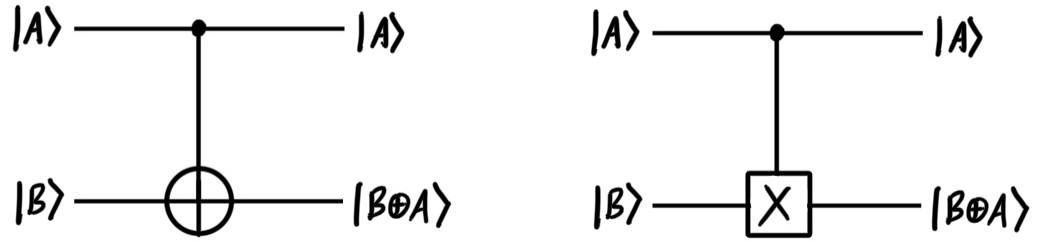
\includegraphics[scale=0.3]{img/Control_Not_gate.jpg}
        \end{center}

        \item The \textbf{controlled-U} gate is a generalization of controlled-NOT. Let us have a control bit and $n$ target bits. If the control bit is set to $|0 \rangle$, then the target qubits are left alone. If the control qubit is set to $|1\rangle$, then the states/spins of the $n$ target qubits are changed by some unitary matrix $U \in \text{U}(2^n)$.

          \[U_{CU} = \begin{pmatrix} I & 0 \\ 0 & U \end{pmatrix}.\]

        Its circuit is represented in the given image.

        \begin{center}
          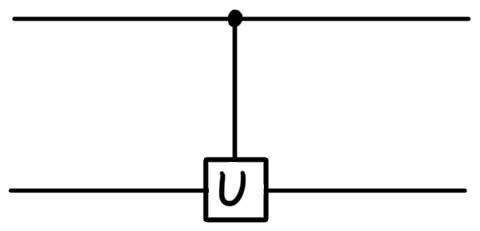
\includegraphics[scale=0.3]{img/Control_U_gate.jpg}
        \end{center}

        \item The \textbf{swap} gate simply swaps the states of the two qubits.

            \[U_{SWAP} = \begin{pmatrix} 1&0&0&0\\0&0&1&0\\0&1&0&0\\0&0&0&1 \end{pmatrix},\]

          and transforms the quantum state

            \[a |00\rangle + b |01\rangle + c|10\rangle + d|11\rangle \mapsto a |00\rangle + c |01\rangle + b|10\rangle + d|11\rangle,\]

          also written

            \[\begin{pmatrix} \alpha_1 \\ \beta_1 \end{pmatrix} \otimes \begin{pmatrix} \alpha_2 \\ \beta_2 \end{pmatrix} = \begin{pmatrix} \alpha_1 \alpha_2 \\ \alpha_1 \beta_2 \\ \beta_1 \alpha_2 \\ \beta_1 \beta_2 \end{pmatrix} \implies U_{SWAP} \begin{pmatrix} \alpha_1 \alpha_2 \\ \alpha_1 \beta_2 \\ \beta_1 \alpha_2 \\ \beta_1 \beta_2 \end{pmatrix} = \begin{pmatrix} \alpha_1 \alpha_2 \\ \beta_1 \alpha_2 \\ \alpha_1 \beta_2 \\ \beta_1 \beta_2 \end{pmatrix} = \begin{pmatrix} \alpha_2 \\ \beta_2 \end{pmatrix} \otimes \begin{pmatrix} \alpha_1 \\ \beta_1 \end{pmatrix}.\]

          Its circuit is represented in the given image.

          \begin{center}
            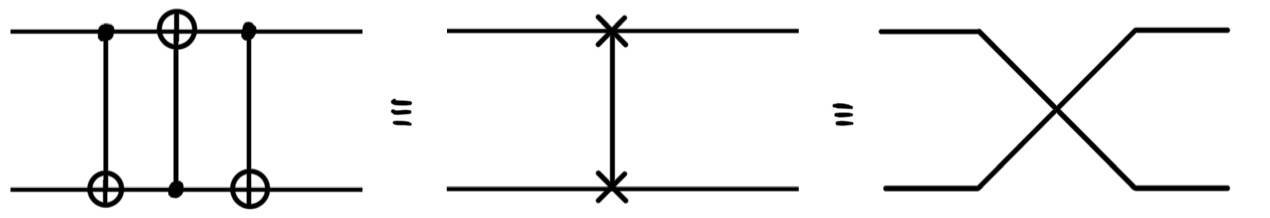
\includegraphics[scale=0.3]{img/Swap_Gate.jpg}
          \end{center}

        \item The \textbf{Toffoli} gate is similar to a CNOT but with two control qubits and 1 target qubit. If the control qubits are set to $|11\rangle$, then the target qubit is flipped.

          \[T = \begin{pmatrix} 1&0&0&0&0&0&0&0\\ 0&1&0&0&0&0&0&0\\ 0&0&1&0&0&0&0&0\\ 0&0&0&1&0&0&0&0\\ 0&0&0&0&1&0&0&0\\ 0&0&0&0&0&1&0&0\\ 0&0&0&0&0&0&0&1\\ 0&0&0&0&0&0&1&0 \end{pmatrix},\]

        and transforms the quantum state

          \begin{align*}
            a|000\rangle & + b|001\rangle + c|010\rangle + d |011\rangle + e|100\rangle + f |101\rangle + g|110\rangle + h|111\rangle \\
            \mapsto & a|000\rangle + b|001\rangle + c|010\rangle + d |011\rangle + e|100\rangle + f |101\rangle + h|110\rangle + g|111\rangle.
          \end{align*}

          Its circuit is represented in the given image.

          \begin{center}
            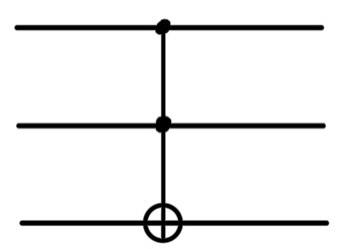
\includegraphics[scale=0.3]{img/Toffoli_gate.jpg}
          \end{center}
      \end{enumerate}

      Finally, we introduce the operation of "measurement," which we represent by a meter symbol.

      \begin{center}
        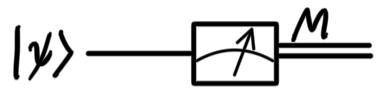
\includegraphics[scale=0.3]{img/Measurement_gate.jpg}
      \end{center}

      This operation converts a single qubit state $| \psi \rangle = \alpha |0\rangle + \beta |1\rangle$ into a probabilistic classical bit $M$, which is $0$ with probability $|\alpha|^2$ or $1$ with probability $|\beta|^2$. 

\section{Quantum Circuits}

  \subsection{No-Cloning Theorem: Copying Bits and Qubits}

    Let us step back into the world of classical computing with classical bits. It is important to know that the CNOT and Toffoli gates take in \textit{quantum bits}, not just classical ones.

    \begin{enumerate}
      \item The classical analogue of the CNOT gate is the XOR gate (or mathematically speaking, XOR is the restriction of CNOT to qubits in superposition of $|0\rangle$ or $|1\rangle$). One of the reasons that XOR is significant is because it can be used as a FANOUT gate, which takes in an arbitrary classical bit $0$ or $1$ and essentially copies it to output $00$ or $11$, where each copy can be used for separate purposes. In the general case, the XOR gate maps

        \[\text{XOR}: \; (A, B) \mapsto (A, A \oplus B),\]

      where $A$ and $B$ are classical bits. By setting the first bit to be some arbitrary $A \in \{|0\rangle, |1\rangle\}$ that we want to copy and the second bit $B = 0$ as a "scratchpad" bit, we have 

        \[\text{XOR}: \; (A, 0) \mapsto (A, A \oplus 0 = A).\]

      \item The Toffoli gate can also be used as a FANOUT gate to copy classical bits since given classical bits $A, B, C$, the Toffoli gate maps 

        \[\text{Toffoli}: \; (A, B, C) \mapsto (A, B, C \oplus A B),\]

      where $A, B, C$ are classical bits. By setting the first bit $A = 1$, $B$ as an arbitrary bit to clone, and $C=0$, we have 

        \[\text{Toffoli}: \; (1, B, 0) \mapsto (1, B, 0 \oplus 1\cdot B = B).\]
    \end{enumerate}

    We have just demonstrated that it is very much possible to clone a classical bit $0$ or $1$, i.e. a quantum bit in a superposition of $|0\rangle$ or $|1\rangle$. However, it turns out that we cannot copy a qubit in some general state $|\psi\rangle = \alpha |0\rangle + \beta |1\rangle$. Attempting a fanout with

    \begin{enumerate}
      \item a CNOT gate by inputting $|\psi \rangle \otimes |0\rangle$, we get

        \[U_{CNOT} \begin{pmatrix} \alpha \\ \beta \end{pmatrix} \otimes \begin{pmatrix} 1 \\ 0 \end{pmatrix} = \begin{pmatrix} 1&0&0&0\\0&1&0&0\\0&0&0&1\\0&0&1&0 \end{pmatrix} \begin{pmatrix} \alpha \\ 0 \\ \beta \\ 0 \end{pmatrix} = \begin{pmatrix} \alpha \\ 0 \\ 0 \\ \beta \end{pmatrix} = \alpha |00\rangle + \beta |11\rangle,\]

      which is not equal to $|\psi \rangle \otimes |\psi \rangle = \alpha^2 |00\rangle + \alpha \beta |01 \rangle + \alpha \beta |10 \rangle + \beta^2 |11 \rangle$. No copying is done.

      \item a Toffoli gate by inputting $|1\rangle \otimes |\psi \rangle \otimes |0\rangle$, we get

        \[T \begin{pmatrix} 0 \\ 1 \end{pmatrix} \otimes \begin{pmatrix} \alpha \\ \beta \end{pmatrix} \otimes \begin{pmatrix} 1 \\ 0 \end{pmatrix} = T \begin{pmatrix} 0\\0\\0\\0\\ \alpha \\ 0 \\ \beta \\ 0 \end{pmatrix} = \begin{pmatrix} 0\\0\\0\\0\\ \alpha \\ 0 \\ 0 \\ \beta \end{pmatrix} = \alpha |100\rangle + \beta |111\rangle,\]

      which is not equal to $|1\rangle \otimes |\psi \rangle \otimes |\psi\rangle = \alpha^2 |000\rangle + \alpha \beta |001 \rangle + \alpha \beta |010\rangle + \beta^2 |011\rangle$. No copying is done.
    \end{enumerate}

    It turns out that it is impossible to copy a qubit with gates, formally stated in the \textbf{No-Cloning theorem}.

  \subsection{Bell States and Quantum Teleportation}

    We introduce the following circuit that takes in two qubits in states $|x\rangle$ and $|y\rangle$, represented as $|xy\rangle$: the $x$-qubit goes through the Hadamard gate and then as the control qubit for the CNOT gate, with the $y$-qubit as the target qubit.

    \begin{center}
      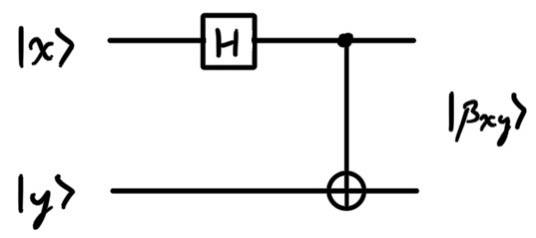
\includegraphics[scale=0.3]{img/Bell_state_circuit_generator.jpg}
    \end{center}

    If we set $|xy\rangle$ as the four computational basis states $|00\rangle, |01\rangle, |10\rangle, |11\rangle$, we get the following \textbf{Bell states}, or \textbf{EPR states}:

    \begin{align*}
      |\beta_{00} \rangle & = \frac{|00\rangle + |11\rangle}{\sqrt{2}}, \\
      |\beta_{01} \rangle & = \frac{|01\rangle + |10\rangle}{\sqrt{2}}, \\
      |\beta_{10} \rangle & = \frac{|00\rangle - |11\rangle}{\sqrt{2}}, \\
      |\beta_{11} \rangle & = \frac{|01\rangle - |10\rangle}{\sqrt{2}},
    \end{align*}

    which are 4 different entangled states of 2 qubits.

    \textbf{Quantum teleportation} is a technique for moving quantum states around. More specifically, suppose A has a qubit in quantum state $|\psi \rangle = \alpha |0\rangle + \beta |1 \rangle$ and wants to send this qubit to B (by "sending" it to B, we mean that we want B to be in possession of a qubit in state $|\psi \rangle$ in some way). This is possible under very special circumstances:

    \begin{enumerate}
      \item An EPR pair (two qubits in some Bell state) has been generated with each qubit given to A and B.

      \item A can communicate to B by sending classical information to B (i.e. finite strings of $0$ and $1$). The finiteness of this condition is most restrictive, since if A could send infinite strings, A can just send the infinite binary representation of $|\psi\rangle$.
    \end{enumerate}

    Under these conditions, this kind of teleportation is called \textbf{entanglement-assisted teleportation}. A can perform the following steps to send $|\psi \rangle$ to B. Let us represent the state to be teleported as $|q_1 \rangle = |\psi\rangle = \alpha |0\rangle + \beta |1\rangle$. A $|q_1 \rangle$ and one EPR pair, which we denote as $|q_2\rangle$, and B has the other EPR pair denoted $|q_3\rangle$.

    \begin{center}
      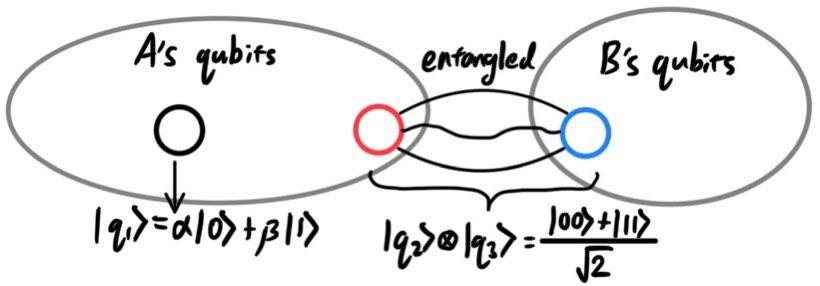
\includegraphics[scale=0.3]{img/Quantum_teleportation.jpg}
    \end{center}

  \begin{enumerate}
    \item The 3-qubit system is in the state

      \[|\psi_0 \rangle = |q_1 \rangle \otimes |q_2 \rangle \otimes |q_3 \rangle = |\psi \rangle \otimes \frac{|00\rangle + |11\rangle}{\sqrt{2}}\]

    which can be written as 

    \begin{align*} 
      |\psi_0 \rangle = |\psi \rangle \otimes |\beta_{00}\rangle & = \big( \alpha |0\rangle + \beta |1\rangle \big) \otimes \frac{1}{\sqrt{2}} \big( |00\rangle + |11\rangle \big) \\
      & = \frac{1}{\sqrt{2}} \Big( \alpha |0\rangle \otimes (|00\rangle + |11\rangle ) + \beta |1\rangle \otimes (|00\rangle + |11\rangle )\Big) \\
      & = \frac{1}{\sqrt{2}} \Big( \alpha |000\rangle + \alpha |011\rangle + \beta |100\rangle + \beta |111\rangle\Big) \\
      & = \frac{1}{\sqrt{2}} \big( \alpha |00\rangle \otimes |0\rangle \big)
    \end{align*}
    
    \item A first sends the 2 qubits $|q_1 \rangle \otimes |q_2 \rangle$ through a CNOT gate, obtaining 

    \begin{align*} 
      |\psi_1 \rangle & = \frac{1}{\sqrt{2}} \big( \alpha |00\rangle \otimes |0\rangle + \alpha |01\rangle \otimes |1\rangle + \beta |11\rangle \otimes |0\rangle + \beta |10\rangle \otimes |1\rangle \big) \\
      & = \frac{1}{\sqrt{2}} \big( \alpha |0\rangle \otimes |00\rangle + \alpha |0\rangle \otimes |11\rangle + \beta |1\rangle \otimes |10\rangle + \beta |1\rangle \otimes |01\rangle \big)
    \end{align*}
    
    \item A sends the first qubit $|q_1\rangle$ through a Hadamard gate, obtaining: 

    \begin{align*}
      |\psi_2 \rangle & = \frac{1}{\sqrt{2}} \bigg( \alpha \frac{|0\rangle + |1\rangle}{\sqrt{2}} \otimes |00\rangle + \alpha \frac{|0\rangle + |1\rangle}{\sqrt{2}} \otimes |11\rangle + \beta \frac{|0\rangle - |1\rangle}{\sqrt{2}} \otimes |10 \rangle + \beta \frac{|0\rangle - |1\rangle}{\sqrt{2}} \otimes |01 \rangle \bigg) \\
      & = \frac{1}{2} \Big( \alpha (|0\rangle + |1\rangle) \otimes (|00\rangle + |11\rangle) + \beta (|0\rangle - |1\rangle) \otimes (|10\rangle + |01\rangle)\Big) \\
      & = \frac{1}{2} \Big( |00\rangle \otimes (\alpha |0\rangle + \beta |1\rangle ) + |01\rangle \otimes (\alpha |1\rangle + \beta |0\rangle) + |10\rangle \otimes (\alpha |0\rangle - \beta |1\rangle ) + |11\rangle \otimes (\alpha |1\rangle - \beta |0\rangle )\Big)
    \end{align*}

    This equation represents the joint distribution of the 3 qubits $q_1 \otimes q_2 \otimes q_3$. For instance, there is a $\Big(\frac{1}{2} \Big)^2 = \frac{1}{4}$ probability of getting $|0\rangle \otimes |0\rangle \otimes (\alpha |0\rangle + \beta |1\rangle)$. Taking the conditional also allows us to interpret this system as having the probabilities: 

    \begin{align*} 
      \mathbb{P}(q_3 = \alpha|0\rangle + \beta |1\rangle \,|\, q_1 \otimes q_2 = |0\rangle \otimes |0\rangle) &= 1 \\
      \mathbb{P}(q_3 = \alpha|1\rangle + \beta |0\rangle \,|\, q_1 \otimes q_2 = |0\rangle \otimes |1\rangle) &= 1 \\
      \mathbb{P}(q_3 = \alpha|0\rangle - \beta |1\rangle \,|\, q_1 \otimes q_2 = |1\rangle \otimes |0\rangle) &= 1 \\
      \mathbb{P}(q_3 = \alpha|1\rangle - \beta |0\rangle \,|\, q_1 \otimes q_2 = |1\rangle \otimes |1\rangle) &= 1
    \end{align*}

    It is clear that B's post-measurement qubit state $q_3$ is completely determined by the post-measurement state of A's teleporting qubit $q_1$ and entangled qubit $q_2$. For instance, if A measures $q_1 \otimes q_2$ to get $|00\rangle$, B will have $q_3 = \alpha |0\rangle + \beta |1\rangle$ with probability $1$. All B has to do now is find A's measurement outcome and adjust its $q_3$ state accordingly to get the original $|\psi\rangle$, by applying the proper gate: 

    \begin{itemize}
      \item A measures $|00\rangle \implies $ B has $|q_3\rangle = \alpha |0\rangle + \beta |1\rangle \xrightarrow{\text{apply }I} \alpha |0\rangle + \beta |1\rangle$. 
      \item A measures $|01\rangle \implies $ B has $|q_3\rangle = \alpha |1\rangle + \beta |0\rangle \xrightarrow{\text{apply }X} \alpha |0\rangle + \beta |1\rangle$. 
      \item A measures $|10\rangle \implies $ B has $|q_3\rangle = \alpha |0\rangle - \beta |1\rangle \xrightarrow{\text{apply }Z} \alpha |0\rangle + \beta |1\rangle$. 
      \item A measures $|11\rangle \implies $ B has $|q_3\rangle = \alpha |1\rangle - \beta |0\rangle \xrightarrow{\text{apply }X \text{ then } Z} \alpha |0\rangle + \beta |1\rangle$. 
    \end{itemize}
    \end{enumerate}

    Note that A must communicate to B the measurement outcome of $|q_1 q_2 \rangle$ over a classic communication channel in order to complete the teleportation. Since this classic information is subject to the limits of speed of light, the teleportation of a qubit does not violate the upper limit. This example may also look like it has violated the No-Cloning theorem, since we have copied the qubit $|\psi\rangle$ from A to B. This is not true, since A's $|q_1\rangle$ qubit collapsed onto either a $|0\rangle$ or $|1\rangle$ upon measurement during the process of teleportation (and so we are left with exactly one copy $|\psi\rangle$ in B's possession).

\section{Quantum Algorithms and Information}

  \subsection{Constructing Reversible Quantum Gates as Extensions of Classical Gates}

    One procedure that we will see is taking a non-reversible, classical gate, which is realized as some function $G: \{0, 1\}^n \longrightarrow \{0, 1\}^m$ and constructing an injective extension $G^*$ of $G$ onto a broader domain and codomain, thereby making it reversible. Note that a reversible gate does not necessarily need to be surjective.

    An example is if we have a one-bit gate $G: \{0, 1\} \longrightarrow \{0, 1\}$ defined $G(0) = G(1) = 1$, then $G$ is clearly not injective. However, we can construct an extension (by extending the codomain to a 2-bit output) defined $G^*: \{0, 1\} \longrightarrow \{0, 1\}^2$ with $G^*(0) = 00, G^*(1) = 10$.

    \begin{center}
      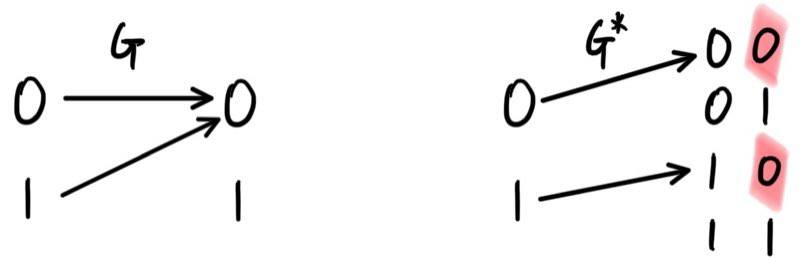
\includegraphics[scale=0.3]{img/Extension_of_G.jpg}
    \end{center}

    $G^*$ now represents a perfectly reversible gate, and it simulates $G$ since all we have to do is look at the second (classical) bit of the output of $G^*$. That is, defining $\delta_2: xy \mapsto x$, we have
    \begin{align*}
      G(0) & = \delta_2 \circ G^* (0), \\
      G(1) & = \delta_2 \circ G^* (1).
    \end{align*}
    What we have essentially done is "distinguished" the $0$ gotten from $G(0)$ and the $0$ gotten from $G(1)$ by attaching a label in front to get $00$ and $10$. The Toffoli gate can simulate the NAND gate as its extension.

    \begin{center}
      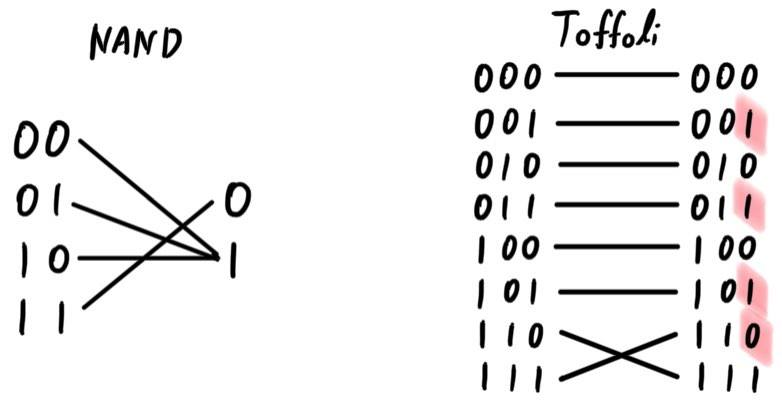
\includegraphics[scale=0.3]{img/Toffoli_NAND_extension.jpg}
    \end{center}

    In order to simulate the NAND gate on input $xy$, we input $xy1$ into the Toffoli and look at the value of the third bit of the output. That is,

      \[\text{NAND}(xy) = \delta_3 \circ \text{Toffoli}(xy1),\]

    where $\delta_3: xyz \mapsto z$. Since the Toffoli gate allows us to simulate the universal NAND gate, it becomes possible to simulate all other elements in a classical circuit and thus an arbitrary classical circuit can be simulated by an equivalent reversible circuit.

  \subsection{Quantum Parallelism}

    Quantum parallelism is a fundamental feature of many quantum algorithms that, heuristically, allows quantum computers to evaluate a function $f(x)$ for many different values of $x$ simultaneously.

    \subsubsection{Function of One-Bit Input}

      Suppose $f: \{0, 1\} \longrightarrow \{0, 1\}$ is a function. To evaluate $f$ on all possible bits, we need to call $f$ 2 times: $f(0), f(1)$. We can create a reversible extension of this function $f$ by extending the domain and codomain to $\{0, 1\}^2$ to construct

        \[U_f: \{0, 1\}^2 \longrightarrow \{0, 1\}^2, \; U_f: \, |x \rangle |y\rangle \mapsto |x\rangle |y \oplus f(x) \rangle.\]

      It may be hard to see why this map $U_f$ is guaranteed to be reversible for all functions $f$, so we will demonstrate with one example of $f$. With the construction of $U_f$ shown below, all we need to do is pay attention to all the outputs where the input has $y=0$, since $U_f (|x \rangle |0\rangle) = |x \rangle \, |f(x) \rangle$.

      \begin{center}
        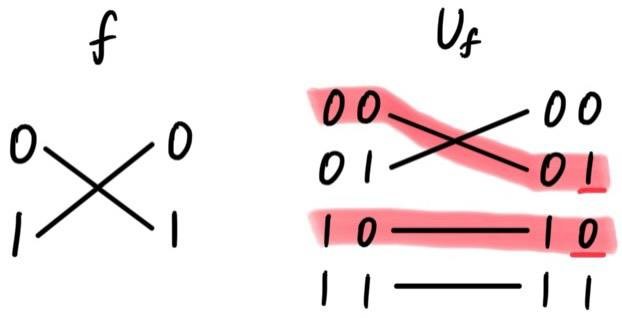
\includegraphics[scale=0.3]{img/f_to_U_one_qubit_reversible.jpg}
      \end{center}

      $U_f$ can also be interpreted to be a quantum gate with qubit inputs rather than classical bits. Since $U_f$ has matrix representation

        \[\begin{bmatrix} 0&1&0&0\\ 1&0&0&0\\ 0&0&1&0\\ 0&0&0&1 \end{bmatrix},\]

      which represents the transformation of the quantum state

        \[a |00\rangle + b|01\rangle + c|10\rangle + d|11\rangle \mapsto b |00\rangle + a|01\rangle + c|10\rangle + d|11\rangle,\]

      So, setting $|y\rangle = |0\rangle$, we can input into $U_f$ the two qubits (more accurately, their composite superposition):

        \[|x \rangle \otimes |y\rangle = \frac{|0\rangle + |1\rangle}{\sqrt{2}} \otimes |0\rangle,\]

      (which can be gotten by applying the Hadamard transform $H$ to $|0\rangle$ and then tensoring $|y\rangle$) to get

      \begin{align*}
        U |x\rangle \otimes |0\rangle & = \frac{1}{\sqrt{2}} U \big( |0\rangle + |1\rangle \big) \otimes |0\rangle \\
        & = \frac{1}{\sqrt{2}} U \big( |00\rangle + |10\rangle \big) \\
        & = \frac{1}{\sqrt{2}} \big( |0\rangle \otimes |f(0)\rangle + |1\rangle \otimes |f(1)\rangle \big).
      \end{align*}

      This output state is very interesting because the different terms contain information about both $f(0)$ and $f(1)$. It is almost as if we evaluated $f(x)$ for two values of $x$ simultaneously. Note that unlike classical parallelism, where multiple circuits each built to compute $f(x)$ are executed simultaneously, here a single $f(x)$ circuit is employed to evaluate the function for multiple values of $x$ simultaneously.

      \subsubsection{Function of Two-Bit Input}

      Suppose $f: \{0, 1\}^2 \longrightarrow \{0, 1\}$ is a function. To evaluate $f$ on all four permutations of two bits, we need to call $f$ 4 times: $f(00), f(01), f(10), f(11)$. We can create a reversible extension of this function $f$ by extending the domain and codomain to $\{0, 1\}^3$ to construct

        \[U_f: \{0, 1\}^3 \longrightarrow \{0, 1\}^3, \;\; U_f: \, |x_1 x_2 \rangle\,|y\rangle \mapsto |x_1 x_2 \rangle\, |y \oplus f(x_1 x_2) \rangle.\]

      It may be hard to see why this map $U_f$ is guaranteed to be reversible for all functions $f$, so we will demonstrate with one example of $f$. With the construction of $U_f$ shown below, all we need to do is pay attention to all the outputs where the input has $y=0$, since $U_f (|x_1 x_2 \rangle |0\rangle) = |x_1 x_2 \rangle \, |f(x) \rangle$.

      \begin{center}
        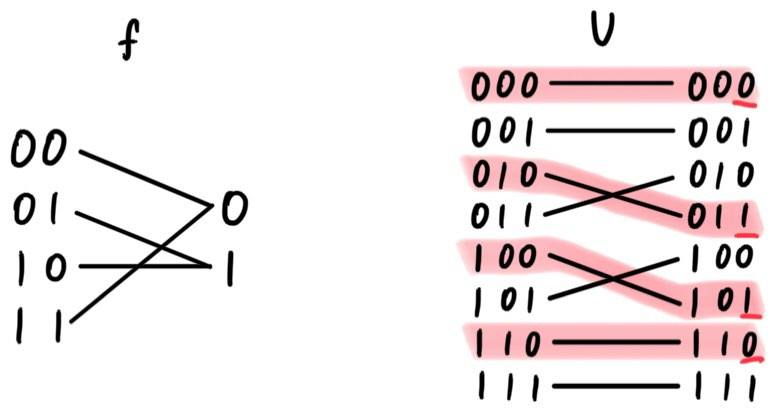
\includegraphics[scale=0.3]{img/f_to_U_reversible.jpg}
      \end{center}

      $U_f$ can also be interpreted to be a quantum gate with qubit inputs rather than classical bits. Since $U_f$ has matrix representation

        \[\begin{bmatrix} 1&0&0&0&0&0&0&0\\0&1&0&0&0&0&0&0\\0&0&0&1&0&0&0&0\\0&0&1&0&0&0&0&0\\0&0&0&0&0&1&0&0\\0&0&0&0&1&0&0&0\\0&0&0&0&0&0&1&0\\0&0&0&0&0&0&0&1 \end{bmatrix},\]

      this represents the transformation of the quantum state

      \begin{align*}
        a|000\rangle & + b|001\rangle + c|010\rangle + d |011\rangle + e|100\rangle + f |101\rangle + g|110\rangle + h|111\rangle \\
        \mapsto & a|000\rangle + b|001\rangle + d|010\rangle + c |011\rangle + f|100\rangle + e |101\rangle + g |110\rangle + h|111\rangle.
      \end{align*}

      So, setting $|y\rangle = |0\rangle$, we can input into $U_f$ the three qubits (more accurately, their composite superposition)

        \[|x_1 x_2 \rangle \otimes |y\rangle = \frac{|0\rangle + |1\rangle}{\sqrt{2}} \otimes \frac{|0\rangle + |1\rangle}{\sqrt{2}} \otimes |0\rangle, \]

      (which can be gotten by applying the Hadamard transform $H^{\otimes 2}$ to $|00\rangle$ and then tensoring $|y\rangle$) to get

      \begin{align*}
        U\,|x_1 x_2 \rangle \otimes |0\rangle & = \frac{1}{2} U \big( |00\rangle + |01\rangle + |10\rangle + |11\rangle \big) \otimes |0\rangle \\
        & = \frac{1}{2} U \big(|000\rangle + |010\rangle + |100\rangle + |110\rangle \big) \\
        & = \frac{1}{2} \big( |00\rangle \otimes |f(00)\rangle + |01\rangle \otimes |f(01)\rangle + |10\rangle \otimes |f(10)\rangle + |11\rangle \otimes |f(11)\rangle \big).
      \end{align*}

      This output state is very interesting because the terms contain information about all $f(00), f(01), f(10)$ and $f(11)$. It is almost as if we evaluated $f(x)$ for four values of $x$ simultaneously.

      \subsubsection{Function of Multiple-Bit Input}

      We can generalize this to an arbitrary number of bits $|x_1 \ldots x_n\rangle \in \{0, 1\}^n$. That is, given some function $f: \{0, 1\}^n \longrightarrow \{0, 1\}$, we can take the state $|0\rangle^{\otimes (n+1)}$ and apply the Hadamard transformation $H^{\otimes n}$ on the first $n$ qubits to prepare the $(n+1)$-qubit state 

        \[|x_1 \ldots x_n \rangle \otimes |y\rangle = \left( \frac{|0\rangle + |1\rangle}{\sqrt{2}}\right)^{\otimes n} \otimes |0\rangle.\]

      Then, we put it through the (reversible) quantum circuit $U_f: \{0, 1\}^{n+1} \longrightarrow \{0, 1\}^{n+1}$ constructed as an extension of the classical $f$ defined 

        \[U_f \, |x_1 x_2 \ldots x_n \rangle \, |y\rangle \mapsto |x_1 x_2 \ldots x_n \rangle \, |y \oplus f(x_1 \ldots x_n)\rangle,\]

      which gives 

        \[U_f \left( \frac{|0\rangle + |1\rangle}{\sqrt{2}}\right)^{\otimes n} \otimes |0\rangle = \frac{1}{\sqrt{2^n}} \sum_{x \in \{0, 1\}^n} |x\rangle \, |f(x)\rangle.\]

      This output state contains information about all of the possible values $f(x)$. But the question still remains what to do with this output 

        \[\frac{1}{\sqrt{2^n}} \sum_{x \in \{0, 1\}^n} |x\rangle \, |f(x)\rangle.\]

      While this one state contains all the information defining the function $f$ on the one hand, it is still in superposition that will collapse onto \textit{one} measurement outcome $|x \rangle \otimes |f(x) \rangle$. Therefore, quantum computation requires something more than just quantum parallelism to be useful; it requires the ability to \textit{extract} information about more than one value of $f(x)$ from superposition states.

  \subsection{Deutsch's Algorithm}

    Given a one-bit input function $f: \{0, 1\} \longrightarrow \{0, 1\}$ and its corresponding reversible extension $U_f: |x\rangle |y\rangle \mapsto |x \rangle |y \oplus f(x)\rangle$, we would like to determine whether this function $f$ is surjective or not. That is, does $f(0)$ and $f(1)$ have the same value or different values? With a classic computer, this will require us to compute $f$ two times (i.e., construct a circuit which must be run twice), but with a quantum one, it requires only one running of a circuit. It is described by the circuit below:

    \begin{center}
      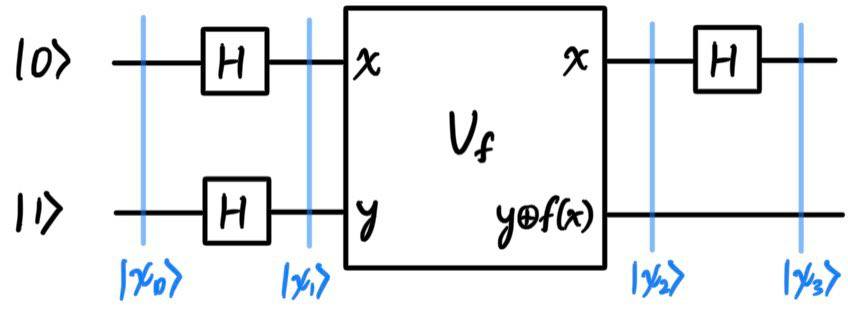
\includegraphics[scale=0.3]{img/Deutsch_Algo.jpg}
    \end{center}

    we start with the input $|0 \rangle \otimes |1\rangle$ and do the following calculations:

    \begin{align*} 
      |\psi_0 \rangle &= |0 \rangle \otimes |1\rangle \\
      &\longmapsto |\psi_1 \rangle = (H \otimes H) |\psi_0 \rangle = \frac{|0\rangle + |1\rangle}{\sqrt{2}} \otimes \frac{|0\rangle - |1\rangle}{\sqrt{2}} \\
      &\longmapsto |\psi_2 \rangle = U_f |\psi_1 \rangle = \begin{cases} 
      \pm \frac{|0\rangle + |1\rangle}{\sqrt{2}} \frac{|0\rangle - |1\rangle}{\sqrt{2}} & \text{if } f(0) = f(1), \\
      \pm \frac{|0\rangle - |1\rangle}{\sqrt{2}} \frac{|0\rangle - |1\rangle}{\sqrt{2}} & \text{if } f(0) \neq f(1),
      \end{cases} \\
      &\longmapsto |\psi_3 \rangle = (H \otimes I) |\psi_2 \rangle = \begin{cases} 
      \pm |0\rangle \frac{|0\rangle - |1\rangle}{\sqrt{2}} & \text{if } f(0) = f(1), \\
      \pm |1\rangle \frac{|0\rangle - |1\rangle}{\sqrt{2}} & \text{if } f(0) \neq f(1).
    \end{cases}
    \end{align*}

    Some clarifications in the calculations:

    \begin{enumerate}
      \item Note that in order to calculate $|\psi_2 \rangle$, we use the fact that
      \begin{align*} 
        U_f |x\rangle \otimes \frac{|0\rangle - |1\rangle}{\sqrt{2}} &= |x\rangle \otimes \left(\frac{|0\rangle - |1\rangle}{\sqrt{2}} \oplus f(x)\right) \\
        &= \begin{cases} 
        |x\rangle \otimes \frac{|0\rangle - |1\rangle}{\sqrt{2}} & \text{if } f(x) = 0, \\
        |x\rangle \otimes \frac{|1\rangle - |0\rangle}{\sqrt{2}} & \text{if } f(x) = 1,
        \end{cases} \\
        &= (-1)^{f(x)}  |x\rangle \frac{|0\rangle - |1\rangle}{\sqrt{2}}.
      \end{align*}
    \end{enumerate}

    Finally, using the fact that $f(0) \oplus f(1) = 0$ iff $f(0) = f(1)$ and $f(0) \oplus f(1) = 0$ otherwise, we can rewrite the above as 

      \[|\psi_3 \rangle = \pm |f(0) \oplus f(1) \rangle \frac{|0\rangle - |1\rangle}{\sqrt{2}}.\]

    Therefore, by measuring just the first qubit of the output system, we can determine $f(0) \oplus f(1)$, i.e., whether $f(0) = f(1)$ or $f(0) \neq f(1)$. This is an amazing property since we can figure this out using just \textit{one} evaluation of $f(x)$, which is impossible with a classical computer that requires at least two evaluations (calculate $f(0)$ and then $f(1)$).

  \subsection{The Deutsch-Jozsa Algorithm}

    A more general algorithm deals with \textbf{Deutsch's problem}. Alice selects a number $x$ from $0$ to $2^n - 1$, which can be represented as an element in $\{0, 1\}^n$ (isomorphic?) and mails it in a letter to Bob. Bob calculates some function $f: \{0, 1\}^n \longrightarrow \{0, 1\}$ and replies with the result, which is either $0$ or $1$. Bob promises to use a function $f$ which is one of two kinds: 

    \begin{enumerate}
      \item $f(x)$ is constant for all values of $x$, or

      \item $f(x)$ is balanced, meaning that it outputs $1$ for exactly half of the possible $x$ and $0$ for the other half (note that this does \textit{not} mean that $f$ outputs $0$ and $1$ probabilistically; $f$ is completely deterministic). 
    \end{enumerate}

    In the classical case, Alice may send Bob one value of $x$ in each letter. At worst, she will need to query Bob at least $2^{n-1} + 1$ times (half of possible inputs, plus one) and therefore the best deterministic classical algorithm she can use therefore requires $2^{n-1} + 1$ queries (i.e. a computational complexity of $O(2^n)$). 

    If Bob and Alice were able to exchange qubits instead of classical bits, and Bob agreed to calculate $f(x)$ using a unitary transformation $U_f$, then Alice can achieve her goal of just \textit{one} correspondence with Bob, using the following algorithm described by the circuit below: 

    \begin{center}
      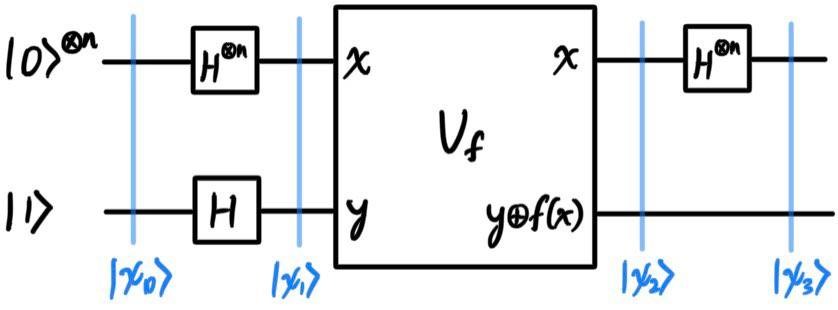
\includegraphics[scale=0.3]{img/Deutsch_Jozsa_Algo.jpg}
    \end{center}

    We start with the $(n+1)$-qubit input $|0\rangle^{\otimes n} \otimes |1\rangle$ and do the following calculations. Remember that in this diagram, Alice sends $|\psi_1\rangle$ to Bob and gets back $|\psi_2\rangle$. 

    \begin{align*} 
      |\psi_0 \rangle = |0\rangle^{\otimes n} \otimes |1\rangle & \longmapsto |\psi_1 \rangle = (H^{\otimes n} \otimes H) |\psi_0 \rangle = \left( \bigotimes_{n} \frac{|0\rangle + |1\rangle}{\sqrt{2}} \right) \otimes \frac{|0\rangle - |1\rangle}{\sqrt{2}} \\ 
      & \;\;\;\;\;\;\;\;\;\;\;\;\;\;\;\;\;\;\;\;\;\;\;\;\;\;\;\;\;\;\;\;\;\;\;\;\;\;\;\;\;\;\;\, = \left( \sum_{x \in \{0, 1\}^n} \frac{1}{\sqrt{2^n}} |x\rangle \right) \otimes \frac{|0\rangle - |1\rangle}{\sqrt{2}} \\
      & \longmapsto |\psi_2 \rangle = U_f |\psi_1\rangle = \sum_{x \in \{0,1\}^n} (-1)^{f(x)} \frac{|x\rangle}{\sqrt{2^n}} \otimes \frac{|0\rangle - |1\rangle}{\sqrt{2}} \\
      & \longmapsto |\psi_3 \rangle = (H^{\otimes n} \otimes I) |\psi_2 \rangle = \sum_{z \in \{0, 1\}^n} \sum_{x \in \{0, 1\}^n} \frac{1}{2^n}\, (-1)^{x \cdot z + f(x)} \,|z\rangle \otimes \frac{|0\rangle - |1\rangle}{\sqrt{2}} 
    \end{align*}

    where $x \cdot z$ is the bitwise dot product of $x, z \in \{0, 1\}^n$ modulo $2$. Some clarifications:

    \begin{enumerate}
      \item Again, to calculate $|\psi_2 \rangle$, we use the fact (which does not matter how many bits $x$ is)

        \[U_f |x\rangle \otimes \frac{|0\rangle - |1\rangle}{\sqrt{2}} = (-1)^{f(x)} \,|x\rangle \, \frac{|1\rangle - |0\rangle}{\sqrt{2}},\]

      and sum it over all possible permutations of $x \in \{0, 1\}^n$ to get 

      \begin{align*} 
        U_f |\psi_1 \rangle & = U_f \left( \sum_x \frac{1}{\sqrt{2}} |x\rangle \right) \otimes \frac{|0\rangle - |1\rangle}{\sqrt{2}} \\
        & = U_f \sum_x \left( \frac{1}{\sqrt{2}} |x\rangle \otimes \frac{|0\rangle - |1\rangle}{\sqrt{2}}\right) \\
        & = \sum_x \frac{1}{\sqrt{2}} U_f \left( |x\rangle \otimes \frac{|0\rangle - |1\rangle}{\sqrt{2}} \right) \\
        & = \sum_x (-1)^{f(x)} \frac{|x\rangle}{\sqrt{2^n}} \otimes \frac{|0\rangle - |1\rangle}{\sqrt{2}}
      \end{align*}

      \item $|\psi_3 \rangle$ is calculated with the following steps. We can see that for $|x\rangle = |0\rangle$ or $|1\rangle$, 

        \[H|x\rangle = \sum_{z \in \{0, 1\}} \frac{1}{\sqrt{2}} (-1)^{xz} |z\rangle = \frac{|0\rangle + (-1)^x |1\rangle}{\sqrt{2}}\]

      Now given an $x = x_1 x_2 \ldots x_n$, we take the tensor products of these terms to get 

      \begin{align*} 
        H^{\otimes n} |x\rangle = H^{\otimes n} \left( \bigotimes_i |x_i \rangle \right) & = H|x_1\rangle \otimes H|x_2\rangle \otimes \ldots \otimes H|x_n\rangle \\
        & = \sum_{z_1 \in \{0, 1\}} \frac{1}{\sqrt{2}} (-1)^{x_1 z_1} |z_1 \rangle \otimes \ldots \otimes \sum_{z_n \in \{0, 1\}} \frac{1}{\sqrt{2}} (-1)^{x_n z_n} |z_n \rangle \\
        & = \frac{1}{\sqrt{2^n}} \sum_{z_1, \ldots, z_n \in \{0, 1\}} (-1)^{x_1 z_1} |z_1 \rangle \otimes \ldots \otimes (-1)^{x_n z_n} |z_n\rangle \\
        & = \frac{1}{\sqrt{2^n}} \sum_{z_1, \ldots, z_n \in \{0, 1\}} (-1)^{x_1 z_1 + \ldots + x_n z_n} \, |z_1 \ldots z_n \rangle \\
        & = \frac{1}{\sqrt{2^n}} \sum_{z \in \{0, 1\}^n} (-1)^{x \cdot z} \, |z\rangle
      \end{align*}

      Therefore, we get 

      \begin{align*} 
        |\psi_3 \rangle & = (H^{\otimes n} \otimes I) |\psi_2 \rangle = H^{\otimes n} \left( \sum_{x \in \{0, 1\}^n} (-1)^{f(x)} \frac{|x\rangle}{\sqrt{2^n}} \right) \otimes I \left( \frac{|0\rangle - |1\rangle}{\sqrt{2}} \right)\\
        & = \left( \sum_{x \in \{0, 1\}^n} \frac{(-1)^{f(x)}}{\sqrt{2^n}} H^{\otimes n} |x\rangle \right) \otimes \frac{|0\rangle - |1\rangle}{\sqrt{2}} \\
        & = \sum_{x \in \{0, 1\}^n} \frac{(-1)^{f(x)}}{\sqrt{2^n}} \left( \frac{1}{\sqrt{2^n}} \sum_{z \in \{0, 1\}^n} (-1)^{x \cdot z} |z \rangle \right) \otimes \frac{|0\rangle - |1\rangle}{\sqrt{2}} \\
        & = \sum_{x \in \{0, 1\}^n} \sum_{z \in \{0, 1\}^n} \frac{1}{2^n} (-1)^{x \cdot z + f(x)} |z\rangle \otimes \frac{|0\rangle - |1\rangle}{\sqrt{2}} \\
        & = \sum_{z \in \{0, 1\}^n} \sum_{x \in \{0, 1\}^n} \frac{1}{2^n} (-1)^{x \cdot z + f(x)} |z\rangle \otimes \frac{|0\rangle - |1\rangle}{\sqrt{2}}
      \end{align*}
    \end{enumerate}

    After applying the Hadamard operator $H^{\otimes n}$ to Bob's result $|\psi_2 \rangle$, Alice is now left with 

      \[|\psi_3 \rangle = \sum_{z \in \{0, 1\}^n} \sum_{x \in \{0, 1\}^n} \frac{1}{2^n} (-1)^{x \cdot z + f(x)} |z\rangle \otimes \frac{|0\rangle - |1\rangle}{\sqrt{2}}. \]

    Alice now observes the query register (i.e., the first $n$ qubits)

      \[\sum_{z \in \{0, 1\}^n} \sum_{x \in \{0, 1\}^n} \frac{(-1)^{x \cdot z + f(x)}}{2^n} |z\rangle = \left( \sum_{x \in \{0, 1\}^n} \frac{(-1)^{f(x)}}{2^n}\right) |0\ldots 0 \rangle \otimes \frac{|0\rangle - |1\rangle}{\sqrt{2}} + \ldots. \]

    Note that the amplitude for the state $|0\rangle^{\otimes n}$ (i.e., when $|z\rangle = |0 \ldots 0\rangle$) is 

      \[\sum_{x \in \{0, 1\}^n} \frac{(-1)^{f(x)}}{2^n}.\]

    There are two scenarios: 
    \begin{enumerate}
      \item If $f(x)$ is constant for all values of $x$, then this amplitude would be 

      \begin{align*} 
        \sum_{x \in \{0, 1\}^n} \frac{(-1)^{f(x)}}{\sqrt{2^n}} & = \sum_{x \in \{0, 1\}^n} \frac{1}{2^n} = 1 \text{ if } f(x) = 0, \\
        \sum_{x \in \{0, 1\}^n} \frac{(-1)^{f(x)}}{\sqrt{2^n}} & = \sum_{x \in \{0, 1\}^n} \frac{-1}{2^n} = -1 \text{ if } f(x) = 1.
      \end{align*}

      Since $|\psi_3 \rangle$ must be a unit vector, this implies that all the other amplitudes are $0$ and therefore $|\psi_3 \rangle = |0\rangle^{\otimes n}$. 

      \item If $f(x)$ is balanced, then the number of negative terms and positive terms will cancel each other out, and so 

        \[\sum_{x \in \{0, 1\}^n} \frac{(-1)^{f(x)}}{2^n} = 2^{n-1} \cdot 1 + 2^{n-1} \cdot (-1) = 0,\]

      meaning that the amplitude of $|0\rangle^{\otimes n}$ is $0$. 
    \end{enumerate}

    Therefore, by measuring these amplitudes Alice can determine whether $f$ is constant or balanced. However, this problem is not known to have any applications, and probabilistic computation can be similarly used to solve this problem with a high (but not certain) degree of accuracy. 

    Remember that quantum computation is superior to classical computation if \textit{both} of the following requirements are met: 

    \begin{enumerate}
      \item We can utilize the non-binary superpositions of qubits to calculate more efficiently using quantum parallelism. 
      \item We have some method to \textit{extract} information from the output qubit(s) using measurements. The answers are all there in the qubit state, but they are hidden: measuring it would cause it to collapse onto a string of $|0\rangle$s and $|1\rangle$s, and so a creative method of gaining information is needed. 
    \end{enumerate}

\section{Quantum Fourier Transform}


\section{Quantum Search Algorithms}


\section{Quantum Computers: Physical Realization}


\section{Quantum Noise and Quantum Operations}


\section{Distance Measures for Quantum Computation}


\section{Quantum Error-Correction}


\section{Entropy and Information}


\section{Quantum Information Theory}


\end{document}
